% ISS presentation template
%
% Change history:
% 24.06.2010    J�rgen Ruoff        Initial creation
% 01.07.2010    Patrick H�cker      Generalization
% 02.07.2010    Patrick H�cker      Adjustment
% 15.11.2010    Patrick H�cker      Improvements
% 20.05.2011    Patrick H�cker      Add presentation type
% 06.01.2012	P. Hermannst�dter 	Adapted to ISS, small mods
% \graphicspath{ {../Fig/} }
% Insert your name here
\newcommand{\presenter}{Zhuowei Han}
\newcommand{\presentershort}{Z.Han}
\newcommand{\presenteremail}{fef} 		% can be accessed using \presenteremail
\newcommand{\x}{\mathbf{x}}
\newcommand{\mX}{\mathbf{X}}
\newcommand{\mH}{\mathbf{H}}
\newcommand{\h}{\mathbf{h}}
\newcommand{\btheta}{\boldsymbol{\theta}}
\newcommand{\y}{\mathbf{y}}
\newcommand{\W}{\mathbf{W}}
\newcommand{\vb}{\mathbf{b}}
\newcommand{\vc}{\mathbf{c}}
\newcommand{\txtcolb}[1]{\textcolor{blue}{\Large #1}}
\newcommand*\OK{\ding{51}}


% Insert presentation title here
\newcommand{\presentationtitle}{Deep Network for Speech Emotion Recognition}
\newcommand{\shortpresentationtitle}{Deep Learning}

% Insert type of presentation here (or comment line), probably one of:
% Mitarbeitervortrag, Bachelor-Arbeit, Master-Arbeit, Bachelor thesis, Master thesis
\newcommand{\presentationtype}{Master Thesis}

% Insert presentation date here
\newcommand{\presentationdate}{16/04/2015}

% Uncomment the following line, if you write in English
%\newcommand{\lang}{german}

% Uncomment the following line, if you want to create handouts (setting to false does not work!)
% \newcommand{\handoutmode}{true}

% Load beamer class using LSS style
% Default \lang to ngerman
\ifx\lang\undefined
	\newcommand{\lang}{ngerman}
\fi

% Set \handout dependant on \handoutmode
\ifx\handoutmode\undefined
	\newcommand{\handout}{}
\else
	\newcommand{\handout}{handout}
\fi

% Make additional colors available
\PassOptionsToPackage{x11names}{xcolor}

% Load the beamer class, set the presentation data and use the LSS layout
\documentclass[\lang,\handout]{beamer}
\author[\presentershort]{\presenter}
\title[\shortpresentationtitle]{\presentationtitle}
\ifx \presentationtype \undefinded
\else
	\subtitle{\presentationtype}
\fi
\date{\presentationdate}
\institute{Institut f�r Signalverarbeitung\\und Systemtheorie\\\vspace{1em}Universit�t Stuttgart}
\usetheme[alternativetitlepage=true,% Use the fancy title page.
          titlepagelogo=isslogocolor,% Logo for the first page.
          watermark=isslogocolor,% Watermark used in every page.
          watermarkheight=25px,% Height of the watermark.
          ]{LSS}

% Grays uncovered objects instead of making them invisible; comment to make uncovered objects invisible
\setbeamercovered{transparent}

% Set work to presentation to not get blue hyperlinks
\newcommand{\work}{presentation}

% Input general definitions and loading of packages which can be shared with the thesis.
% Comment this line if you want to decide yourself which packages should be loaded.
% \def\me{Patrick H�cker}

% this is needed to get more resources to TeX - otherwise not all packages work at the same time
\usepackage{etex}

% erm�glicht ein if-then-else in LaTeX z. B. um Pakete variabel einzubinden
\usepackage{xifthen}
% \newcommand{\ifthen}[1]{\ifthenelse{#1}{}} % It does not work (behaviour is wrong)

% Load language specific things. Always load german, too, to get things like the long name of LSS correctly.
\ifx\lang\undefined
	\newcommand{\lang}{ngerman}
\fi
\ifthenelse{\equal{\lang}{german}}{
	\renewcommand{\lang}{ngerman}
}{}

\ifthenelse{\not\equal{\lang}{ngerman}}{
	\usepackage[ngerman,\lang]{babel}
}{
	\usepackage[\lang]{babel}
}

% damit man Umlaute direkt eingeben kann und diese erkannt werden (sp�ter auf utf8 umsteigen).
\usepackage[x-iso-8859-1]{inputenx}

% Umlaute werden als eine Einheit angesehen -> richtige Trennung und korrekt ins PDF eingebunden;
\usepackage[T1]{fontenc}

% Enth�lt gewisse Sonderzeichen wie z. B. Bullets
\usepackage{textcomp}

% Allow more set symbols (does not replace amsmath symbols if included before amsmath)
\usepackage[bbgreekl]{mathbbol}

% Schaltet AMS-Befehle, Schriftzeichen und Symbole frei (Mathepaket)
% Allow bold uppercase greek letters using the boldsymbol command
\usepackage{amsmath}
\usepackage{amsfonts}
\usepackage{amssymb}

% Allows bold italic uppercase letters
\usepackage{fixmath}



%Erlaubt den Seitenumbruch in Formeln, auch wenn er nach M�glichkeit vermieden wird
\allowdisplaybreaks[4]

% Enables fraction of the form a/b (with a nice slash)
\usepackage{nicefrac}

% Bindet die standardm��ig genutzten Times-Fonts ein (muss nach amsmath eingebunden werden)
% \usepackage{txfonts}

% Uses the Latin Modern font
\usepackage{lmodern}

% erm�glicht die aufrechte Schreibung griechischer Buchstaben
\usepackage{upgreek}

%erm�glicht das Einbinden von EPS-Dateien
\usepackage{graphicx}

%Das nachtr�gliche �ndern von Texten und Anpassen der Schriftart in EPS-Dateien beim Einbinden
\usepackage{psfrag}

%erm�glicht farbigen Text
\usepackage[x11names]{xcolor}

%erm�glicht farbige Tabellenhintergr�nde
\usepackage{colortbl}

% tikz is a cool drawing package using pgf
\usepackage{tikz}

\usetikzlibrary{3d,arrows,automata,backgrounds,calc,calendar,chains,decorations,decorations.footprints,decorations.fractals,decorations.markings,decorations.pathmorphing,decorations.pathreplacing,decorations.shapes,decorations.text,er,fadings,fit,folding,matrix,mindmap,patterns,petri,plothandlers,plotmarks,positioning,scopes,shadows,shapes.arrows,shapes.callouts,shapes,shapes.gates.logic.IEC,shapes.gates.logic.US,shapes.geometric,shapes.misc,shapes.multipart,shapes.symbols,through,topaths,trees}

% pgfplots enables the simple creation of plots from data points (eg. generated by matlab2tikz.m)
\usepackage{pgfplots}

% save every tikz plot as a pdf file (see package documentation of pgfplots)
% \usepgfplotslibrary{external}
% \tikzexternalize{ the main file name }

% If you want to print on a different size, use this package temporally
% \usepackage{pgfpages}
% \pgfpagesuselayout{resize}[a3paper]

% set PGF's decimal separator to comma for german documents
\ifthenelse{\equal{\lang}{ngerman}}{
	\pgfkeys{/pgf/number format/.cd, set decimal separator={{{,}}}}
}{}

% damit kann man Diagramme und Funktionen zeichnen
% \usepackage{pstricks,pst-plot,pst-node}
%\usepackage{pstricks-add}

% Zugriff auf gnuplot aus LaTeX heraus (erfordert -shell-escape bei latex-Aufruf)
% \usepackage{gnuplottex}

%\usepackage{multicol}

% Introduces \vref, a command which adds the page to the reference if necessary
\usepackage{nameref}
\usepackage{varioref}

\ifthenelse{\equal{\work}{thesis} \OR \equal{\work}{paper}}{
	\ifthenelse{\equal{\version}{computer}}{
		\def\colortype{color}
	}{}
	\ifthenelse{\equal{\version}{print}}{
		\def\colortype{black}
	}{}

	% Macht Links und Referenzen farbig und entfernt h�ssliche K�stchen drumherum
	% Hyperlinks blau ('color') (=PC-Version) oder schwarz ('black') (=Druckversion)
	\ifthenelse{\equal{\colortype}{color}}{
		\usepackage[breaklinks=true,colorlinks,linkcolor=blue]{hyperref}
	}{
		\usepackage[breaklinks=true]{hyperref}
	}
}
{
	\usepackage{hyperref}
}

% Makes the boolean ifpdf available to check if LaTeX is directly generating a PDF file


\usepackage{ifpdf}

\ifpdf
\else
	% Sorgt daf�r, dass \url-Befehl automatische Umbr�che unterst�tzt (macht Probleme mit pdflatex)
	\usepackage{breakurl}
\fi

% Erm�glicht Abbildungen, die vom Text umflossen werden
% (zwei unterschiedliche Ans�tze, haben wohl beide Nachteile)
% \usepackage{floatflt}
\usepackage{wrapfig}

% Setzt manche Bildunterschriften n�her ans Bild heran, was sch�ner aussieht
\usepackage[hang]{caption}

% mehrere kleine Tabellen oder Grafiken aneinander anordnen (muss nach caption eingebunden werden)
%\usepackage{subfig}

%\usepackage{subfloat}

% Sauber formatierte Quellcode-Umgebung zur Verf�gung stellen
\usepackage{listings}

% Erm�glicht Tabellen, deren Gesamtbreite eingestellt werden kann, wobei eine Spalte �brigen Platz bekommt
\usepackage{tabularx}

% Erm�glicht Tabellen, deren Gesamtbreite eingestellt werden kann, wobei �briger Platz prozentual aufgeteilt wird
\usepackage{tabulary}

% Erstellt sch�nere Tabellen, wobei vertikale Linien nicht mehr benutzt werden d�rfen
\usepackage{booktabs}

% Erm�glicht Tabellenzellen die Ausdehnung �ber mehrere Zeilen
\usepackage{multirow}

% Writes an additional file to enable backward synchronisation between PDF and LaTeX
% "pdfsync uses extremely sensible code. You should not use pdfsync on final documents because
% it can change the layout rather significantly", yep, I hit a bug
% \usepackage{pdfsync}

% Erm�glicht das hinzuf�gen von fixme-Kommentaren, auch als \todo
\usepackage{fixme}
\newcommand{\todo}[1]{\fxwarning{#1}}
%\usepackage[inline,\status]{fixme}

% Ist f�r die �bergangsphase zu pdflatex sinnvoll, weil dann auch eps-Grafiken eingebunden werden k�nnen
%\usepackage{epstopdf}

% Abk�rzungsverzeichnis erstellen und konfigurieren
%\usepackage[german,intoc]{nomencl}
%\renewcommand{\nomname}{Abk�rzungsverzeichnis}
%\let\abbrev\nomenclature
%\setlength{\nomlabelwidth}{.15\hsize}
%\makenomenclature

% Stellt \doublespacing, \onehalfspacing und \singlespacing zur Verf�gung
\usepackage{setspace}

% Allows putting two images on top of each other
% \usepackage[percent]{overpic}

% The savetrees package packs as much text as possible onto each page
% \usepackage{savetrees}

% Stellt das Kommando \extrarowheight f�r das glossaries-Paket zur Verf�gung
\usepackage{array}

% allows usage of \degree
\usepackage{gensymb}

% Abk�rzungen
% Sets
\newcommand{\Z}{\mathbb{Z}}
\newcommand{\N}{\mathbb{N}}
\newcommand{\Q}{\mathbb{Q}}
\newcommand{\R}{\mathbb{R}}
\newcommand{\C}{\mathbb{C}}

% differentiation
\newcommand{\del}{\partial}
\newcommand{\derivate}[2]{\frac{\del #1}{\del #2}}
\DeclareMathOperator{\dif}{d}
\DeclareMathOperator{\gradlong}{grad}
\DeclareMathOperator{\grad}{\bigtriangledown}

% statistics
\newcommand{\erw}[1]{\operatorname{E}\left(#1\right)}
\DeclareMathOperator{\E}{E}
\DeclareMathOperator{\prop}{P}
\DeclareMathOperator{\Var}{Var}
\DeclareMathOperator{\Cov}{Cov}
\DeclareMathOperator{\Bias}{Bias}
\DeclareMathOperator{\CRB}{CRB}

% linear algebra
\newcommand{\mat}[1]{\mathbf{#1}}
%\newcommand{\mat}[1]{\boldsymbol{#1}}
\newcommand{\Tr}[1]{\mathrm{Tr}\left( #1 \right)} %deprecated
\newcommand{\tr}[1]{\mathrm{tr}\left( #1 \right)}
\newcommand{\rang}[1]{\mathrm{rang}\left( #1 \right)}
\newcommand{\diag}[1]{\mathrm{diag}\left( #1 \right)}
\newcommand{\pinv}[1]{#1^{\dagger}}
\newcommand{\trans}[1]{#1^{\mathrm{T}}}
\newcommand{\hermitian}{\mathrm{H}}
\newcommand{\herm}[1]{#1^\mathrm{H}}
\newcommand{\konj}[1]{#1^{\mathrm{*}}}
\newcommand{\est}[1]{\hat{#1}}
\newcommand{\abs}[1]{\left\lvert#1\right\rvert}
\newcommand{\norm}[1]{\left\lVert#1\right\rVert}

% german abbreviations
\newcommand{\zB}{\mbox{z.\,B. }}
\newcommand{\iA}{\mbox{i.\,A. }}
\newcommand{\deha}{\mbox{d.\,h.\ }}
\newcommand{\oae}{\mbox{o.\,�.\ }}
\newcommand{\uae}{\mbox{u.\,�.\ }}
\newcommand{\oBdA}{\mbox{o.\,B.\,d.\,A. }}
\newcommand{\OBdA}{\mbox{O.\,B.\,d.\,A. }}
\newcommand{\ggf}{\mbox{ggf.\ }}
\newcommand{\vgl}{\mbox{vgl.\ }}
\newcommand{\evtl}{\mbox{evtl.\ }}
\newcommand{\bzw}{\mbox{bzw.\ }}
\newcommand{\bspw}{\mbox{bspw.\ }}
\newcommand{\ca}{\mbox{ca.\ }}

% english abbreviations
\newcommand{\eg}{\mbox{e.g.\ }}
\newcommand{\ie}{\mbox{i.e.\ }}

% quotes
\newcommand{\gq}[1]{\glq#1\grq}
\newcommand{\gqq}[1]{\glqq#1\grqq}
\newcommand{\eq}[1]{`#1'}
\newcommand{\eqq}[1]{``#1''}


% functions
\newcommand{\e}[1]{\operatorname{e}^{\,#1}}
\newcommand{\argmax}[2]{\underset{#1}{\operatorname{argmax}}\left( #2 \right)}
\newcommand{\argmaxima}[2]{\underset{#1}{\operatorname{argmaxima}}\left( #2 \right)}
\newcommand{\argmin}[2]{\underset{#1}{\operatorname{argmin}}\left( #2 \right)}
\DeclareMathOperator{\arc}{arc}
\DeclareMathOperator{\sinc}{sinc}
\DeclareMathOperator{\ggT}{ggT}
\DeclareMathOperator{\kgV}{kgV}
\DeclareMathOperator{\lcm}{lcm}

% symbols
% \newcommand{\degree}{\ensuremath{^\circ}}
\newcommand{\entspricht}{\mathrel{\hat{=}}}
\newcommand{\sollgleich}[0]{\overset{!}{=}}
\newcommand{\help}{\textcircled{\scriptsize{?}}}

% general
\newcommand{\op}[1]{\operatorname{#1}}
\newcommand{\smtext}[1]{{\scriptscriptstyle\text{#1}}}
%Zeilenumbruch mit eineinhalbzeiligem Abstand
\newcommand{\br}{\vspace{0.6em}\newline} %entspricht etwa \par\smallskip, geht aber auch in captions
\newcommand{\unit}[2]{\ensuremath{#1}\,\ensuremath{\mathrm{#2}}}
% \newcommand{\definition}[1]{\textit{#1}}
\newcommand{\includeplot}[1]{\centering\includegraphics{parent/Plots/#1.eps}}
\newcommand{\link}[1]{\href{#1}{\url{#1}}}
\newcommand{\shortlink}[1]{\href{#1}{#1}}
\newcommand{\mailto}[1]{\href{mailto:#1}{#1}}
\newcommand{\textlink}[2]{\href{#2}{\url{#1}}}
\newcommand{\vecfun}[2]{#1\hspace{-0.1em}\left(\vec #2\right)}
\newcommand{\equal}[1]{\overset{\text{#1}}{=}}
\newcommand{\matlab}{\textsc{Matlab}\raisebox{1ex}{\tiny{\textregistered}} }

% renews
\renewcommand{\inf}{\infty}
\renewcommand{\matrix}[1]{\mathbf{#1}}
\renewcommand{\j}{\mathrm{j}}
\renewcommand{\gcd}[0]{\operatorname{gcd}}
\renewcommand{\-}{\,--\,}


% Definiert den Befehl \writetofile, der als erstes Argument den Dateinamen und als zweiten Befehl den zu schreibenden Text erwartet
\newcommand{\writetofile}[2]{
% Erstelle Variable outfile
\newwrite\outfile
%�ffne Datei mit Handle outfile
 \immediate\openout\outfile=#1
%Schreibe in Datei
 \immediate\write\outfile{#2}
%Schlie�e Datei
\immediate\closeout\outfile
}

\newcommand{\readfromfile}[1]{
\newread\infile
\immediate\openin\infile=#1
\immediate\read\infile to \tempXBE
\immediate\closein\infile
\tempXBE
}


% \newcommand{\dotsnewline}{\mydotfill\,\linebreak.}

% Allgemeinerer Ansatz als Paket nomencl um mehrere Abk�rzungs-/Symbolverzeichnisse zu erstellen
% Glossary "acronym" wird vordefiniert und Glorraries kommen in Inhaltsverzeichnis (toc)
% einsetzbar: toclike2, toclike3
%\usepackage[acronym,toc,style=toclike3acronym]{glossaries}
% deactivate toclike3acronym temporally due to squeeze upgrade

% Deactivated here and activated in main document, as makeglossaries does not work otherwise (WTF?)
% \usepackage[acronym,toc,style=listdotted]{glossaries}

% Abschlie�ender Punkt in jeder Zeile wird weggelassen
% \renewcommand{\glspostdescription}{}
% L�sst Leerzeile bei Anfangsbuchstabenwechsel in den Verzeichnissen weg
% \renewcommand{\glsgroupskip}{}

% \newcommand{\newacronymdots}[2]{\newglossaryentry{#1}{type=\acronymtype, name={#1}, description={#2}, text={#1}, first={#2 (#1)}, plural={#1s}, firstplural={#2s (#1s)}, symbol={\dotsnewline}}}


% \newcount\boolcounter
% \boolcounter=1
% \advance\boolcounter by 1
% erm�gliche Kennzeichnung eines Akronyms im Text durch \acronym{was}
%%%\newcommand{\acronym}[1]{\acr{#1}}
% \newcommand{\acronym}[1]{\gls{#1}}
% \let\acronym\gls
% \newcommand{\acronym}[1]{#1}
%\newcommand{\acronymnolink}[1]{\protect\acr*{#1}}
% erm�glicht die Benutzung eins Akronyms mit beliebigem Text (Argument #2)
% \newcommand{\acronymtext}[2]{\glslink{#1}{#2}}
% erm�glicht das Benutzen eines Akronyms, ohne dass die ausgeschriebene Version (dieses Mal) verwendet wird
% \newcommand{\acronymshort}[1]{\glslink{#1}{#1}}
% Verwendet ein Akronym ohne einen Link zu setzen (geht nicht in floating-Umgebungen)
%\newcommand{\acronymnolink}[1]{#1\glsadd{#1}}
% erm�gliche Definition eines Akronyms in akronyme.tex durch \defineacronym{was}{wie}
% \newcommand{\defineacronym}[2]{\newacronym{#1}{#1}{#2}}
% \newcommand{\defineacronym}[2]{}
% \newcommand{\defineacronymdots}[2]{\newacronymdots{#1}{#2}}
%Sorgt daf�r, dass man "\acronym{DoS}[-Angriff]" schreiben kann und dann automatisch "DoS-Angriff (Denial of Service)"
%geschrieben wird, bzw. "DoS-Angriff", je nachdem, ob es das erste Mal ist oder nicht
% \defglsdisplayfirst[acronym]{#3#4 (#2)}
% analog zu Akronymen: \definevar legt Symbol an, \var referenziert dieses
% \let\var\gls
% \newcommand{\var}[1]{#1}
% \newcommand{\var}[1]{\ifodd\boolcounter{%
% \protect\gls*{#1}%
% }\else%
% \text{\gls{#1}}\fi%
% }
%\newcommand{\varshort}[1]{\text{\glslink{#1}}\text{#1}}
%\newcommand{\varquiet}[1]{\glsadd{#1}}
%\newcommand{\definevar}[3]{\newglossaryentry{#1}{name=\ensuremath{#2},description={#3},sort=#1}}
\newcommand{\definevar}[4]{\newglossaryentry{#2}{name=\ensuremath{#3},description={#4},sort=#1}}
% \newcommand{\definevar}[4]{}
%\newcount\varcounter
%\varcounter=1
%\newcommand{\definevar}[3]{\definevariable{#1}{#2}{\arabic\varcounter #3}{\arabic\varcounter}}%{\arabic\varcounter}\advance\varcounter by 1}
%\newcommand{\definevariable}[4]{\newglossaryentry{#1}{name=\ensuremath{#2},description={#3},sort={#4}}\advance\varcounter by 1}
%\newcommand{\definevar}[4][\DefaultOpt]{%
%\def\DefaultOpt{#2}%
%\newglossaryentry{#2}{name=\ensuremath{#3},description={#1 wird sortiert #4},sort=#1}%
%\newglossaryentry{#2}{name=\ensuremath{#3},description={#4}}%
%}
% \newcommand{\varnolink}[1]{\protect\gls*{#1}}

% create glossaries internally (deactivated here, as this results in an error, must be activated in main file (WTF?))
% \makeglossaries

% \let\addtocontentsOld\addtocontents
% \renewcommand{\addtocontents}[2]{\advance\boolcounter by 1 \addtocontentsOld{#1}{#2} \advance\boolcounter by 1}

%Problem: Hochzahlen sitzen um Variablen mit Index unsauber, tempor�re L�sung:
%\text{\glslink{thetaHatDNF}{$\hat{\vec{\theta}}_{\mathrm{DNF}}^3$}}
%anstatt:
%\var{thetaHatDNF}^3

% unknown hyphenation rules
\hyphenation{Im-puls-ant-wort Im-puls-ant-wort-ko-ef-fi-zien-ten
Pro-gramm-aus-schnitt Mi-kro-fon-sig-nal Sig-nal Rech-ner-ar-chi-tek-tur
Rech-ner-ar-chi-tek-tur-en Leucht-dich-te-mess-ka-me-ra Gam-ma-kor-rek-tur IEEE
Grund-an-nah-me}

% Definiert die Farbe Gray aus gray mit 80% S�ttigung
\definecolor{Gray}{gray}{0.8}

%definiert deutsche hyperref-Bezeichner so um, dass \autoref problemlos funktioniert
% \ifthenelse{\equal{\lang}{ngerman}}{
% 	\addto\extrasngerman{%
% 		\def\appendixautorefname{Anhang}%
% 		\def\chapterautorefname{Kapitel}%
% 		\def\equationautorefname{Gleichung}%
% 		\def\itemautorefname{Punkt}%
% 		\def\pageautorefname{Seite}%
% 		\def\partautorefname{Teil}%
% 		\def\sectionautorefname{Kapitel}%
% 		\def\subsectionautorefname{Kapitel}%
% 		\def\figureautorefname{Abbildung}%
% 		\def\footnoteautorefname{Fu�note}%
% 		\def\tableautorefname{Tabelle}%
% 	}
% }{
% 	\addto\extrasngerman{%
% 		\def\appendixautorefname{Appendix}%
% 		\def\chapterautorefname{Chapter}%
% 		\def\equationautorefname{Equation}%
% 		\def\itemautorefname{Item}%
% 		\def\pageautorefname{Page}%
% 		\def\partautorefname{Part}%
% 		\def\sectionautorefname{Chapter}%
% 		\def\subsectionautorefname{Chapter}%
% 		\def\figureautorefname{Figure}%
% 		\def\footnoteautorefname{Footnote}%
% 		\def\tableautorefname{Table}%
% 	}
% }


% define autoref to act like eqref for equations
\makeatletter
\@ifdefinable\equationname{%
\let\equationname\equationautorefname%
}
\addto\extrasenglish{%
\def\equationautorefname~#1\@empty\@empty\null{(#1\@empty\@empty\null)}
}
% \addto\extrasngerman{%
% \def\equationautorefname~#1\@empty\@empty\null{\equationname~(#1\@empty\@empty\null)}
% }
\makeatother

% Use serifs in math environment and no serifs in text environment
\usefonttheme[onlymath]{serif}

% Define two practical lengths, which can be uses when setting the size of graphics
\newlength\fullwidth
\setlength\fullwidth{11cm}
\newlength\fullheight
\setlength\fullheight{6.8cm}

% Set lines a bit thicker in presentations when using pgfplots to allow recognition of colored lines
\ifx\pgfplotsset\undefined
	%
\else
	\pgfplotsset{every axis/.append style={thick}}
\fi

% Put four slides on each page if handout mode activated
\ifx\handoutmode\undefined
	%
\else
	\usepackage{pgfpages}
	\pgfpagesuselayout{4 on 1}[a4paper,border shrink=5mm,landscape]
	% use this line instead, if you have problems with rotated eps files
	% \pgfpagesuselayout{4 on 1}[border shrink=5mm,landscape]
\fi


% Define Layout parameters:
\setlength{\itemsep}{0.5em}


\usepackage{setspace}
\usepackage{graphicx}
\usepackage{amsmath}
\usepackage{pgfpages}
\usepackage{subfigure}
\usepackage{cancel}
\usepackage{colortbl}
\usepackage{tabularx}
\graphicspath{ {../Fig/} }
\usepackage[beamer]{hf-tikz}
\usepackage{tikz}
\usetikzlibrary{calc}
\usepackage{array,graphicx}
\usepackage{booktabs}
\usepackage{pifont}
\def\layersep{2.5cm}
\def\layersept{5cm}
% \usetikzlibrary{matrix,chains,positioning,decorations.pathreplacing,arrows}
\def\layersep{2.5cm}
% \setbeameroption{show notes on second screen=left}
% \setbeameroption{second mode text on second screen=left}
% \setbeameroption{show notes}
% \setbeameroption{show notes on second screen=left}


% My commands:

% -----------------------------------------------------------------------------
% -----------------------------------------------------------------------------
\begin{document}
\lstset{basicstyle=\small\ttfamily,xleftmargin=15pt,language=Matlab,
        commentstyle=\color{green},showstringspaces=false,stringstyle=\color{magenta}\ttfamily}

% -----------------------------------------------------------------------------
% This is the title page
\begin{frame}[t,plain]
	\titlepage
\end{frame}


% -----------------------------------------------------------------------------
% Motivation slide
% \begin{frame}[t]{Motivation} % 1 folie
% % \textcolor{blue}{\Large Training objective}
% \only<1-1>{
% \textcolor{blue}{\Large Speech Emotion Recognition}\\
% 	\begin{itemize}
% 		\itemsep15pt
% % 		\item Most current work focuses on speech processing based on linguistic information,  e.g.: Skype Translator
% 		\item More natural human-machine interaction requires paralinguistic information such as age, gender, emotion.
% 		\item Emotion is high-dimensional complex data with non-linear time-variant hidden features
% 		\item Traditional feature learning is labor expensive
% % 		\item Speech Recognition / Speeker Identification / Emotion Recognition
% 		\only<1-1>{\begin{figure}[b]
% 		 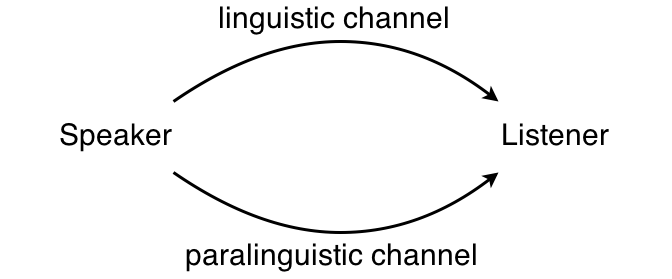
\includegraphics[width=0.6\linewidth]{paraliguistic.png}
% 		\end{figure}}
% 
% 	\end{itemize}
% }
% 
% \only<2-2>{
% \textcolor{blue}{\Large Deep Learning}\\
% 	\begin{itemize}
% 	    \itemsep15pt
% 	    \item New research area of machine learning
% 	    \item Deep architecture for building high-level representations via unsupervised feature learning
% 	    \item Learning both temporal and non-temporal features 
% 	    \item Application in vision/audition processing, e.g. handwriting recognition (Graves, Alex, et al. 2009), traffic sign classification (Schmidhuber, et al. 2011), text translation (Google, 2014)
% 	\end{itemize}
% }
% \end{frame}

% -----------------------------------------------------------------------------
% This is the table of contents. You can insert a motivation before or after this slide.
\begin{frame}
	\ifthenelse{\equal{\lang}{ngerman}}{
		\frametitle{Table of Contents}
	}{
		\frametitle{Table of Contents}
	}
	\tableofcontents
\end{frame}

% Add an extra slide at the beginning of each section while highlighting the current section
% Use \section* to skip the slide once or comment the following to skip all overview slides.
\AtBeginSection[]
{
	\begin{frame}<beamer>
		\ifthenelse{\equal{\lang}{ngerman}}{
			\frametitle{Table of Contents}
		}{
			\frametitle{Table of Contents}
		}
% 		\frametitle{\contentsname}
		\tableofcontents[currentsection]
	\end{frame}
}

%% =========
\section{Foundations} %1 F
% -----------------------------------------------------------------------------
	\begin{frame}[t]{Foundations}
% 	\txtcolb{Mel Frequency Cepstral Coefficients}
% 			\begin{itemize}
% 				\item most commonly used features in speech emotion analysis 
% 				\item short-term power spectrum based on frame
% 				\item mel-scale approximate human perception
% 				\begin{align}
% 				f_{mel} = 1125~\ln~(1+f_{Hz}/700)\nonumber
% 				\end{align}
% 			\end{itemize}
% 
% 		\begin{figure}
% 		 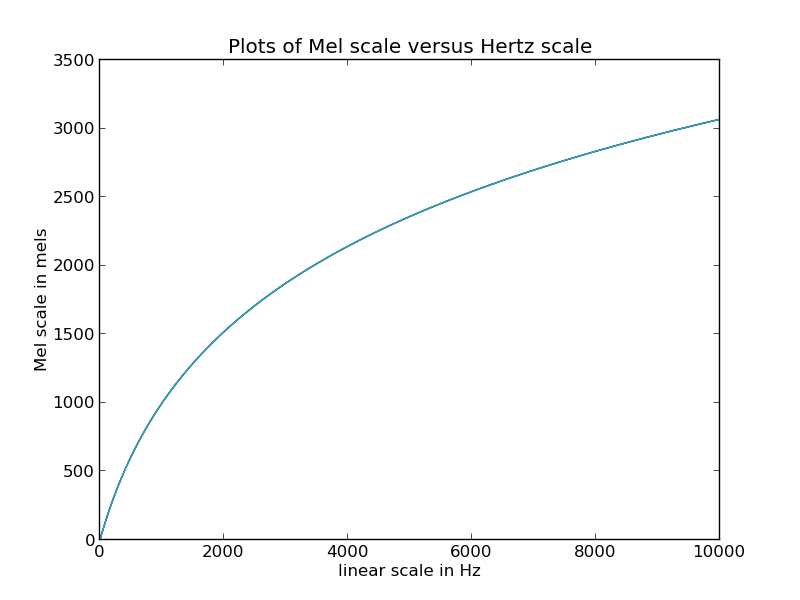
\includegraphics[width = 0.5\linewidth]{MelvsHz.png}
% 		\end{figure}
% 	\end{frame}
% 	
% 	
% 	\begin{frame}[t]{Pre-processing for MFCCs}
% 	\txtcolb{Steps to MFCCs}
% 		      \begin{enumerate}
% 		      \item Convert speech signal with overlapped window to frames ($20ms$ frame length, $10ms$ shifting).
% 		      \item Calculate power spectrum for each frame with DFT and take the logarithm value.
% 		      \item Apply Mel filterbank to the power spectrum, sum the power in each filter.
% 		      \item Decorrelation by applying Discrete Cosine Transform (DCT) to the logarithm of the filter powers.
% 		      \item Keep coefficients $1-20$ of DCT and discard the rest.
% 		      \end{enumerate}
% 
% 		      \begin{figure}[htbp]
% 		      
\includegraphics[width= \textwidth]{mfcc.png}
% 		      \end{figure}
% 	\end{frame}
	
% 	\begin{frame}[t]{Foundations}
	\txtcolb{Framework of Emotion Recognition}
	      \begin{itemize}
	       \item Extract spectrum features: Mel Frequency Cepstral Coefficients
	       \item Aggrogate MFCCs to build high-level representations via unsupervised learning
	       \item Classification based on high-level features via supervised learning
	      \end{itemize}
	      \vspace{10mm}
	      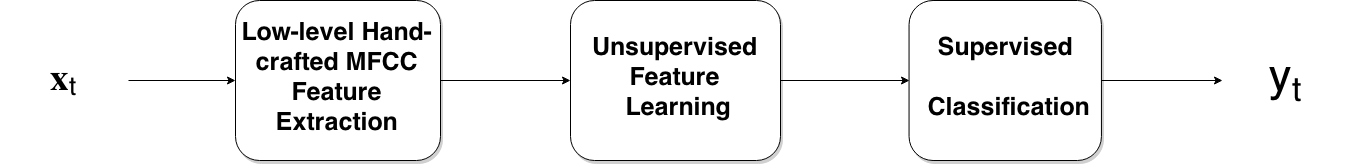
\includegraphics[width=\linewidth]{Framework.png}

	\end{frame}
% 
% 
% % 
% \subsection{Emotion Recognition Approaches}
% 
% \begin{frame}[t]{Emotion Recognition Approaches}
% 	\begin{minipage}[t]{0.48\linewidth}
% 	  \textcolor{blue}{\Large Traditional Approaches}
% 	  \begin{itemize}
% 	   \item pre-selected features
% 	   \item supervised training
% 	   \item low-level features not appropriate for claasification
% 	   \item shallow structure of classifiers
% 	  \end{itemize}
% 	\end{minipage}\hfill
% 	\begin{minipage}[t]{0.48\linewidth}
% 	\textcolor{blue}{\Large Deep Learning Approaches}
% 	  \begin{itemize}
% 	   \item learning representations from high-dim data
% 	   \item extracting appropriate features without hand-crafting
% 	   \item low-level features are used to build high-level features as network gets deeper
% 	   \item frame-based classification
% 	  \end{itemize}
% 
% 	\end{minipage}
% \end{frame}

% %%%%%%%%%%%%%%%%%%%%%%%%%%%%%%%%%%%%%%%%%%%%%%%%%%%%%%%%%%%%%%%%%%%%%%
\section{Conditional Restricted Boltzmann Machine} %% 
\subsection{Restricted Boltzmann Machine}
	\begin{frame}[t]{Conditional Restricted Boltzmann Machine}
	 \begin{itemize}
	  \itemsep10pt
	  \item Energy-based undirected graphical model
	  \item Contains hidden variables (hidden units), increases the modeling capacity.  
	  \item Unsupervised feature learning 
		  \begin{itemize}
		   \item build high-level features from low-level features 
% 		   \item capture data distribution $P^{\btheta}(\x)$
		   \item learned features used for prediction or classification
		  \end{itemize}
	  \item Successfully applied in motion capture (Graham W. Taylor, Geoffrey E. Hinton, 2006)
% 	  \item speicifies a joint distribution over input and hidden variables, can either generating data, or with bayesian
% rule to form conditional distribution. 
% 	  \item non-temporal, but is potential to be extended to capture temporal information
	 \end{itemize}
	\end{frame}
	
	\begin{frame}[t]{Restricted Boltzmann Machine}
	\txtcolb{Structure}
	    \begin{figure}[t]
		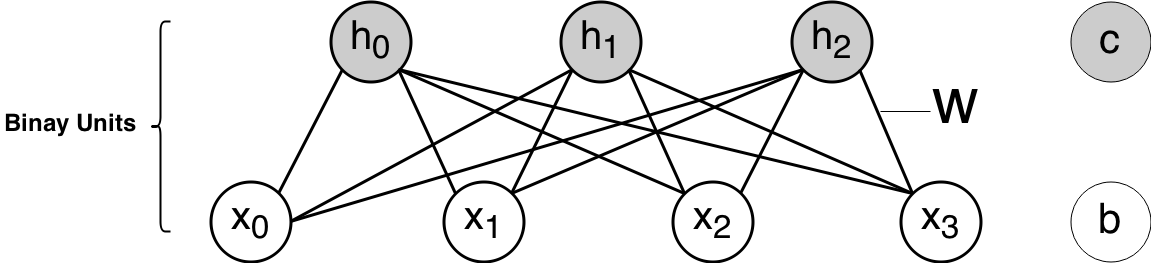
\includegraphics[width=0.9\linewidth]{RBMStruct.png}
	    \end{figure}
	    \only<1-1>
	    {\begin{align}
	      &\text{visible/input layer} &\x \in \{0,1\}\nonumber\\
	      &\text{hidden layer} &\h \in \{0,1\}\nonumber\\
	      &\text{weight} &\mathbf{W}\nonumber\\
	      &\text{visible bias} &\mathbf{b}\nonumber\\
	      &\text{hidden bias} &\mathbf{c}\nonumber\\
	      &\text{parameter set} &\btheta = \{\mathbf{W},\mathbf{b},\mathbf{c}\}\nonumber
	     \end{align}

	    }
	    \only<2->{
	      \begin{minipage}{0.48\linewidth}
	      \begin{align}
		\text{Energy Function:}~&E_{\boldsymbol{\theta}}(\x,\h) = -\mathbf{x^{T}}\mathbf{W}\mathbf{h}-\mathbf{b^{T}}\x-\mathbf{c^{T}}\mathbf{h}\nonumber\\
	      \text{Joint Distribution:}~&P^{RBM} (\x,\mathbf{h}) = \frac{1}{Z} e^{-E_{\boldsymbol{\theta}}(\x,\mathbf{h})}\nonumber\\
	      \text{Partition Function:}~ &Z = \sum_{\mathbf{x,h}} e^{-E_{\boldsymbol{\theta}}(\x,\mathbf{h})}\nonumber\\
	      \text{Free Energy:}~& \mathcal{F}(\x) = - \log \sum_h e^{-E(\mathbf{x,h})}\nonumber
	      \end{align}
	      \end{minipage}
	    }
	\end{frame}
 \subsection{CRBM}
	\begin{frame}[t]{Conditional RBM}
	    \only<1->{
	    \includegraphics<1>[width=0.7\linewidth]{CRBM2.png}
	    \begin{columns}
	    \column{1.5in}
	    \includegraphics<2>[scale = 0.2]{CRBM2.png}
	    \column{2in}
	    \includegraphics<2>[scale = 0.2]{RBMStruct2.png}
	    \end{columns}
	    }
	    \only<1-1>{
	    \begin{itemize}
	     \item Consider visible units from previous time step as additional bias for current visible and hidden layer
% 	     \item $A$ and $B$ are weight parameter of visible (history) - visible and visible (history) - hidden connections
	     \item Visible layer consists of linear units with independent Gaussian noise to model real-valued data, e.g. spectral features
	    \end{itemize}
	    }
	    \only<2->{\begin{align}
	      \text{Energy Function:}~&E^{CRBM}_{\boldsymbol{\theta}} (\x, \mathbf{h})  =\left \| \frac{\x - \tilde{\mathbf{b}}}{2} \right\|^{2}
    -\tilde{\mathbf{c}}^T \mathbf{h}-\x^{T} \mathbf{W}\mathbf{h} \nonumber\\
	      &\tilde{\mathbf{b}} = \mathbf{b} + \mathbf{A}\cdot \x_{<t}\nonumber\\
	      &\tilde{\mathbf{c}} = \mathbf{c} + \mathbf{B}\cdot \x_{<t}\nonumber\\
% 	      & \x_{<t}, ~\mathrm{history input}\nonumber\\
	      &\boldsymbol{\theta} = \{\mathbf{W,A,B},\mathbf{b},\mathbf{c} \}\nonumber\\
	      \text{Free Energy:}~& \mathcal{F}(\x) = - \log \sum_h e^{-E(\mathbf{x,h})}\nonumber
	    \end{align}
	    }


	\end{frame}	
	\begin{frame}[t]{Inference}
	\txtcolb{Inference}
		\begin{minipage}[t]{0.48\linewidth}

			 \begin{align}
			 &P(\x) = \sum_{\mathbf{h}} P(\mathbf{x,h})\nonumber\\ 
			 &P (\mathbf{h}) = \sum_{\x} P(\mathbf{x,h})\nonumber\\
			 &P (\h|\x)= \dfrac{P(\x,\h)}{P(\x)}\nonumber\\
			 &P(\x|\h)= \dfrac{P(\x,\h)}{P(\h)}\nonumber\\
			 &P(h_{j}=1 \mid \x)= sigmoid(\sum_{i} x_{i}W_{ij} + c_{j})\nonumber\\
			 &P(x_{i}=1 \mid \mathbf{h}) = sigmoid(\sum_{j} W_{ij} h_{j} + b_{i})\nonumber
			 \end{align}
		 \end{minipage}
	\end{frame}

	
	\begin{frame}[t]{Training of Energy-based Model}
% 	      \begin{columns}[c]
% 		    \column{3in}
		    \alert<1-1>{Maximum Likelihood Estimation} $P^{\btheta}(\x)$\\\vspace{5mm}
		    \only<2->{
		    \textcolor{blue}{Kullback-Leibler Divergence}:
		    \begin{align}
			Q(\x)\|P^{\btheta}(\x) &=  \int_{-\infty}^{\infty} Q(\x)\cdot \log \dfrac{Q(\x)}{P^{\btheta}(\x)}\mathrm{d}\x \nonumber\\
						& = \int_{-\infty}^{\infty}Q(\x)\cdot\log Q(\x) \mathrm{d} \x - \int_{-\infty}^{\infty}Q(\x)\cdot\log P^{\btheta}(\x) \mathrm{d} \x \nonumber\\
						& = \left \langle \log Q(\x)\right\rangle_{Q(\x)} - \left\langle \alert<3->{\log P^{\btheta}(\x)}\right\rangle_{Q(\x)}\nonumber
		    \end{align}
		    $Q(\x)$, true data distribution\\\vspace{2mm}
		    $P^{\btheta}(\x)$, parameterized distribution, to be estimated\\\vspace{2mm}
		    $\left\langle\cdot\right\rangle_{Q(\x)}$, expectation w.r.t. $Q(\x)$\\\vspace{2mm}
		    }
% 	      \end{columns}
	 \end{frame}

	
	\begin{frame}[t]{Training of Energy-based Model}
		
		\uncover<1-3>{
		\begin{columns}
		 \column{5in}
		      \begin{align}
				- \log P^{\btheta}(\x) = \mathcal{F}(\x) + \log\sum_{\x}\sum_{\h}e^{-E_{\btheta}(\x,\h)}\nonumber
		      \end{align}
% 		\column{1.5in}
% 		Free Energy
		\end{columns}
		}
		
		      \begin{columns}
			    \column{4in}
		\only<1->{  \begin{align}
				    -\frac{\partial  \log P^{\btheta}(\x)}{\partial \boldsymbol{\theta}} = \frac{\partial \mathcal{F}(\x)}{\partial \boldsymbol{\theta}} -
				    \sum_{\tilde{\x}} P(\tilde{\x})
					\frac{\partial \mathcal{F}(\tilde{\x})}{\partial \boldsymbol{\theta}}\nonumber
			    \end{align}
			    $\x$, input (visible) data space\\
			    $\tilde{\x}$, all possible vectors in the data space, generated by model.\vspace{5mm}
			}
		\only<2->
		{objective function by averaging log-likelihood over data:
			    \begin{align}\label{loggra}
				    - \left\langle\frac{\partial  \log P^{\btheta}(\x)}{\partial \boldsymbol{\theta}}\right\rangle_{Q(\x)} = \left\langle \frac{\partial \mathcal{F}(\x)}{\partial \boldsymbol{\theta}}\right\rangle_{Q(\x)} -\alert<3->{
					  \left\langle \frac{\partial \mathcal{F}(\tilde{\x})}{\partial \boldsymbol{\theta}}\right\rangle_{P(\tilde{\x})}\nonumber}
			    \end{align}
		}
% 		      \column{1.5in}
%       % 		\[ \xleftarrow{\hspace*{3mm}} \]
% 		      \textcolor{red}{$\leftarrow$intractable!}
		      \end{columns}

% 		\only<3->{
% 		      \begin{columns}
% 		      \column{3in}
% 			\begin{align}
% 			      - \frac{\partial  \log P^{\btheta}(\x)}{\partial \boldsymbol{\theta}} = \frac{\partial \mathcal{F}(\x)}{\partial \boldsymbol{\theta}} - \alert<3-3>{ \frac{1}{|\mathcal{N}|}
% 			    \sum_{\tilde{\x}\in \mathcal{N}} P(\tilde{\x})
% 				\frac{\partial \mathcal{F}(\tilde{\x})}{\partial \boldsymbol{\theta}}\nonumber}
% 			\end{align}
% 		      \column{1.5in}
% 		      sampling
% 			\end{columns}
% 		  }
	\end{frame}
	
% 	\begin{frame}[t]{Training of Energy-based Model}
% % % 		Sampling Method: \textcolor{red}{Gibbs Sampling}
% 		\txtcolb{Gibbs sampling}
% 		\begin{columns}[c]
% 			  \column{1.5in}
% 			\uncover<1-1>{\begin{align}
% 			      & \x^{(0)} \sim P(\x)\nonumber \\
% 			      & \mathbf{h}^{(0)} \sim P(\mathbf{h}|\x^{(0)})\nonumber	
% 			\end{align}
% 			}
% 			\uncover<2-2>{
% 			\begin{align}
% 				  & \x^{(1)} \sim P(\x|\mathbf{h}^{(0)})\nonumber\\
% 				  & \mathbf{h}^{(1)} \sim P(\mathbf{h}|\x^{(1)})\nonumber
% 			\end{align}
% 			}
% 			\uncover<3-3>{
% 			\begin{align}
% 				& \vdots \nonumber\\
% 				& \x^{(k)} \sim P(\x|\mathbf{h}^{(k-1)})\nonumber	
% 			\end{align}
% 			}
% 
% 			  \column{3in}
% 			  \framebox{\includegraphics<1>[width=\textwidth]{markov_chain.png}
% 				    \includegraphics<2>[width=\textwidth]{markov_chain2.png}
% 				    \includegraphics<3>[width=\textwidth]{markov_chaint.png}
% 				    }
% 		\end{columns}
% % 		\only<2->{
% % 		\begin{columns}[c]
% % 			  \column{1.5in}
% % 
% % 			  \column{1.5in}
% % 			  \framebox{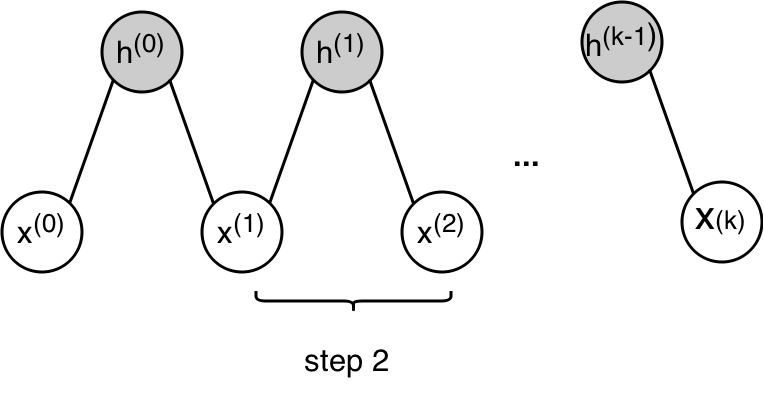
\includegraphics[width=\textwidth]{markov_chain2.png}}
% % 		\end{columns}
% % 		}
% % 		\only<3->{
% % 		\begin{columns}[c]
% % 			  \column{1.5in}
% % 
% % 			  \column{1.5in}
% % 			  \framebox{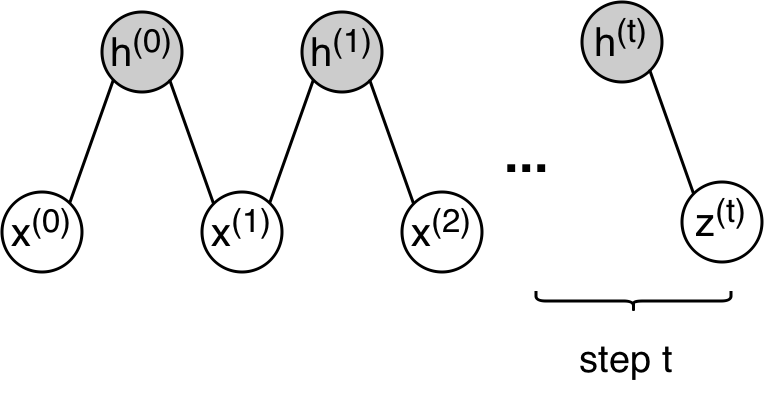
\includegraphics[width=\textwidth]{markov_chaint.png}}
% % 		\end{columns}
% % 		}
% % 		
% % 	\only<4->{$t=1$, Gibbs step $\rightarrow$ \textcolor{red}{Contrastive Divergence}}
% 	\end{frame}
	
	\begin{frame}[t]{Training of Energy-based Model}
% 	 \textcolor{blue}{Contrastive Divergence}\\
	 \txtcolb{Contrastive Divergence} (Hinton)
	 \begin{itemize}
	    \itemsep10pt
	    \only<1-1>{
	    \item Obtain $P(\tilde{\x})$ by Gibbs sampling
	    \item k=0, $P_0(\x) (= Q(\x))$ is true data distribution, independent of parameter $\btheta$
	    \item $ P_{\infty}^{\btheta}(\x) \rightarrow P(\tilde{\x})$
		  \begin{figure}[t]
		  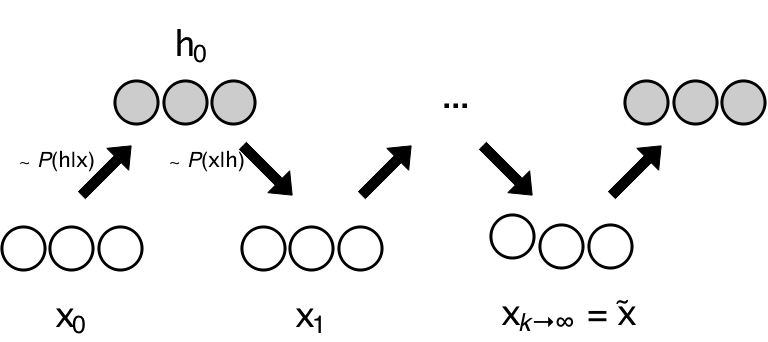
\includegraphics[scale = 0.3]{Gibbs.png}
		  \end{figure}
		  }
	    
	    \only<2->{
	    \item In practise perform 1-Gibbs step will work well:\\
		  \begin{align}
		   - \left\langle\frac{\partial  \log P^{\btheta}(\x)}{\partial \boldsymbol{\theta}}\right\rangle_{P_0(\x)} = \alert<2->{\left\langle \frac{\partial \mathcal{F}(\x)}{\partial \boldsymbol{\theta}}\right\rangle_{P_0(\x)}} -\alert<2->{
					  \left\langle \frac{\partial \mathcal{F}(\x)}{\partial \boldsymbol{\theta}}\right\rangle_{P^{\btheta}_{1}(\x)}\nonumber}
		  \end{align}
		  \begin{figure}
		  \includegraphics<2>[scale = 0.3]{Gibbs1.png}
		  \end{figure}

		\only<3->{\begin{align}
	  \Delta \btheta \sim \left\langle \frac{\partial \mathcal{F}(\x)}{\partial \boldsymbol{\theta}}\right\rangle_{P_0} 
		  -\left\langle \frac{\partial \mathcal{F}(\x)}{\partial \boldsymbol{\theta}}\right\rangle_{P_{1}^{\btheta}}\nonumber
		\end{align}
		}
		}
	 \end{itemize}
	  
	\end{frame}
	
% 	\begin{frame}[t]{Constrasive Divergence}
% 	\txtcolb{Contrastive Divergence} (Hinton):\\
% 	 Perform CD-1
% 	    \begin{align}
% 	    &-\dfrac{\partial}{\partial \btheta} (P_0\|P_{\infty}^{\btheta} - P_{1}^{\btheta}\|P_{\infty}^{\btheta})\nonumber\\\vspace{3mm}
% 	    &=\left\langle \frac{\partial \mathcal{F}(\x)}{\partial \boldsymbol{\theta}}\right\rangle_{P_0} 
% 		  -\left\langle \frac{\partial \mathcal{F}(\x)}{\partial \boldsymbol{\theta}}\right\rangle_{P_{1}^{\btheta}}\nonumber
% % 		  \uncover<1-2>{+ \alert<2-2>{\frac{\partial P_{1}^{\btheta}}{\partial \btheta} \frac{\partial (P_{1}^{\btheta}|P_{\infty}^{\btheta})}{\partial P_{1}^{\btheta}}\nonumber}}
% 		  \uncover<1-2>{ +\alert<2-2>{\frac{\partial P_{1}^{\btheta}}{\partial \btheta} \frac{\partial (P_{1}^{\btheta}|P_{\infty}^{\btheta})}{\partial P_{1}^{\btheta}}\nonumber}}
% 	    \end{align}
% 	    
% 	 \only<3->
% 	 {\txtcolb{Parameter Update}
% 	 \begin{align}
% 	  \Delta \btheta \sim \left\langle \frac{\partial \mathcal{F}(\x)}{\partial \boldsymbol{\theta}}\right\rangle_{P_0} 
% 		  -\left\langle \frac{\partial \mathcal{F}(\x)}{\partial \boldsymbol{\theta}}\right\rangle_{P_{1}^{\btheta}}\nonumber
% 	 \end{align}
% 	}
% 	\end{frame}
% % 
% 
% 
% 
% 
%   
% % % %%%%%%%%%%%%%%%%%%%%%%%%%%%%%%%%%%%%% =========

\section{Deep Neural Network}%4 folies
	\subsection{Function and Training}	
	\begin{frame}[t]{DNN for Classification}
	      \begin{itemize}
		\itemsep10pt
		\item Using high-level features to perform classification
		\item DNN Structure
		      \begin{itemize}
			    \item Feedforward network
			    \item Recurrent network
		      \end{itemize}  
	      \end{itemize}
	 \begin{figure}
	      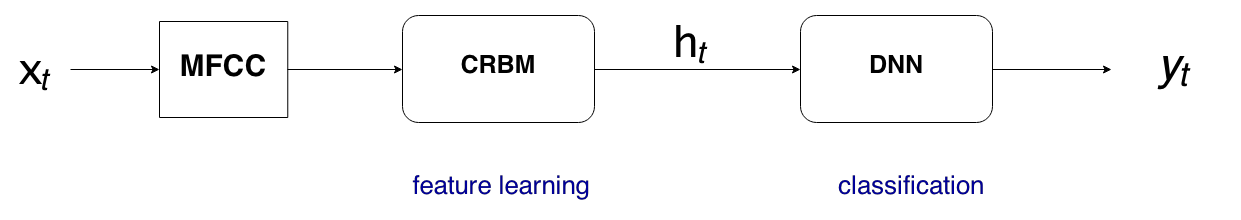
\includegraphics[width=\linewidth]{Framework2.png}
	 \end{figure}
	\end{frame}

	\begin{frame}[t]{Structure and Function}
	  \begin{columns}[T]
	      \column{2in}
	      \txtcolb{Feedforward Structure}
	      Hidden layer pre-activation:
	       \begin{align}
	       \mathbf{a}(\x) =\mathbf{W}^{(1)}\x + \mathbf{b}^{(1)}\nonumber
% 	       a_{j}(\x) = \sum_i w_{ji}^{(1)}x_{i} + b_{j}^{(1)}\nonumber
	       \end{align}
	       Hidden layer activation:
	       \begin{align}
		  \h = f(\mathbf{a})\nonumber
		\end{align}
	  \column{2.5in}
	  		    \tikzset{neuron/.style={circle,thick,fill=black!25,minimum size=17pt,inner sep=0pt},
			input neuron/.style={neuron, draw,thick, fill=gray!30},
			hidden neuron/.style={neuron,fill=white,draw},
			output neuron/.style={neuron,draw,thick,fill=black!20},
			hoz/.style={rotate=-90}}   %<--- for labels

		   \scalebox{0.7}
		   {
		   \begin{tikzpicture}[t,-,draw=black, node distance=\layersep,transform shape,rotate=90,width=0.2\textwidth,height=0.2\textwidth]  %<-- rotate the NN

		    % Draw the input layer nodes
		    \foreach \name / \y in {1/1,3/n}
		    \node[input neuron, hoz] (I-\name) at (0,-\name) {\color{black}$x_\y$};

		    \node[hoz] () at (0,-2) {$\dots$};
		    % Draw the hidden layer nodes
		    \foreach \name / \y in {1/1,2/2,4/\text{\tiny n-1},5/n}
		    \path[yshift=1cm] node [hidden neuron, hoz] (H-\name) at (\layersep,-\name cm) {\color{black}$h_\y$};
		    \node [output neuron, hoz] at (3.8,-5) {\color{black}$\mathbf{b}^{(2)}$};
		    \node [hidden neuron, hoz] at (1.3,-5) {\color{black}$\mathbf{b}^{(1)}$};
		    \path[yshift=1cm]
		      node[hoz] () at (\layersep,-3 cm) {$\dots$};
% 		    \path[yshift=0.5cm]
% 		      node[hoz] () at (\layersep,-5 cm) {$\dots$};


		    %%%%%%%%%% Draw the output layer nodes
		    \foreach \name / \y in {1/1,2/2,3/3,4/4}
		    \path[yshift=0.5cm] node [output neuron, hoz](O-\name) at (\layersept,-\name cm){\color{black}$y_\y$};

		    % 		      \node[output neuron,hoz] () at (\layersept,-3 cm) {$\dots$};
					  
		    \path node[hoz,right] at (1.3,1) {\color{black}$\mathbf{W}^{(1)}$};      
		    \path node[hoz,right] at (3.8,1) {\color{black}$\mathbf{W}^{(2)}$}; 
		    \path node[hoz,right] at (\layersep,-4.5 cm) {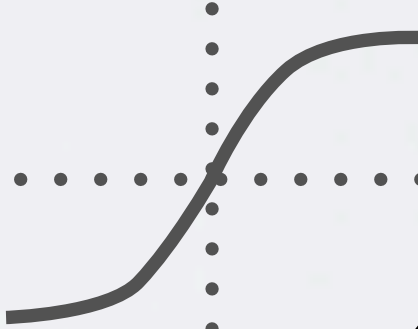
\includegraphics[width=0.2\textwidth]{activation.png}}; 
		    
		    
		    % Connect every node in the input layer with every node in the  hidden layer.
			\foreach \source in {1,3}
			    \foreach \dest in {1,2,4,5}
				\path[->] (I-\source.north) edge (H-\dest.south);
			\foreach \source in {1,2,4,5}
			  \foreach \dest in {1,2,3,4}
			      \path[->] (H-\source.north) edge (O-\dest.south);
		    \end{tikzpicture}
		    }
	  \end{columns}\vspace{5mm}
	  \begin{columns}[T]
	   \column{3in}
		Output layer activation of single hidden layer:
		 \begin{align} 
		 \hat{y}(\x) = o(\mathbf{W}^{(2)}\h^{(1)} + \mathbf{b}^{(2)} )\nonumber
		 \end{align}
		 Output layer activation of $N$ hidden layers:
		 \begin{align} 
		 \hat{y}(\x) = o(\mathbf{W}^{(N+1)}\h^{(N)} + \mathbf{b}^{(N+1)} )\nonumber
		 \end{align}
	    \column{1.5in}
	  \end{columns}

	  
% 	  \begin{minipage}{0.45\linewidth}
% 		\begin{figure}
% 		      \includegraphics{}
% 		\end{figure}
% 	  \end{minipage}

	\end{frame}
	
\begin{frame}[t]{Structure and Function}
	\txtcolb{Recurrent Structure}
	\begin{columns}
	 \column{2in}
	 \begin{align}
				&h_{t} = \mathcal{H}(W_{xh}x_{t}+W_{hh}h_{t-1} + b_{h})\nonumber\\
				&y_{t} = W_{hy}h_{t} + b_{y}\nonumber
			\end{align}
	  \begin{figure}
	  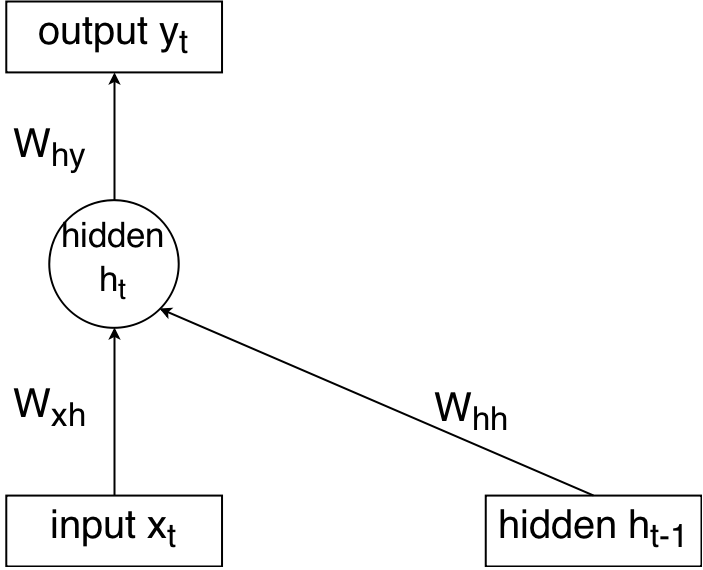
\includegraphics[width=\textwidth]{RNNunit.png}
	  \end{figure}
	 
	\end{columns}
\end{frame}
  
	\begin{frame}[t]{Training}
		\textcolor{blue}{\Large Empirical Risk Minimization}
		\begin{itemize}
		 \item Objective
		 \begin{eqnarray}
			\text{arg}~\underset{\btheta}{\mathrm{min}} \frac{1}{M}\sum_m l(\hat{y}(\x^{(m)};\btheta),y^{(m)}) + \lambda \Omega(\btheta)\nonumber
			\end{eqnarray}
		 \item Loss function $l(\hat{y}(\x^{(m)};\btheta),y^{(m)})$ , $\btheta = \{\mathbf{W},\mathbf{b}\}$
% 			for sigmoid activation $l(\btheta)= \sum_m \frac{1}{2} \left\| y^{(m)}-\hat{y}^{(m)}\right\| ^2$\\
		 \item Regularizer $\lambda \Omega(\btheta)$, L1 \& L2 regularization
		\end{itemize}
		\vspace{5mm}
		\txtcolb{Optimization}
		\begin{itemize}
		 \item Stochastic gradient descent
		 \item Layerwise pre-training \& Backpropagation (BP)
		\end{itemize}

		
		
	\end{frame}
	
	
% 	\subsection{Problems and Solutions}
% 		
% 	\begin{frame}[t]{Unsupervised Layerwise Pre-training}
% 		\begin{minipage}[h]{\linewidth}
% 		\txtcolb{Vanishing Gradient in BP}
% 			\begin{itemize}
% 				\item Training time increases as network gets deeper
% 				\item Gradient shrink exponentially and training end up local minima
% 				\item Caused by random initialization of network parameters
% 			\end{itemize}
% 		\end{minipage}\vspace{5mm}
% 		\begin{minipage}[h]{\linewidth}
% 		\only<1-1>{
% 		\begin{figure}
% 		 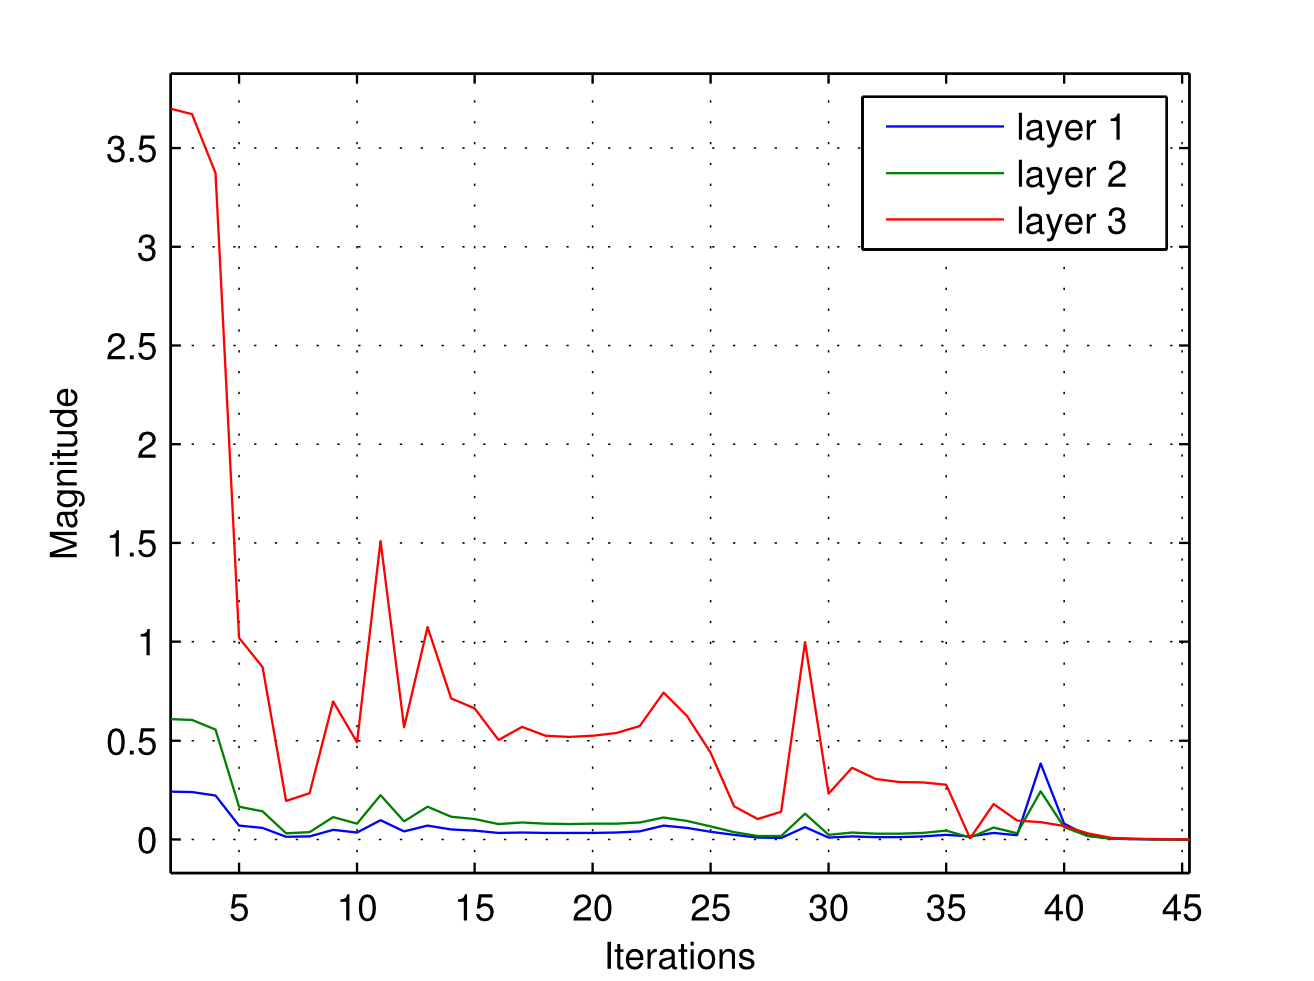
\includegraphics[width=0.6\textwidth]{GradVanishing.png}
% 		\end{figure}
% 
% 		}
% 		\visible<2->{
% 		\txtcolb{Unsupervised layerwise pre-training}
% 		\begin{itemize}
% 		 \itemsep8pt
% 		 \item Pretrain the deep network layer by layer in unsupervised way to build a stacked auto-encoder
% 		 \item Each layer is trained as a single hidden layer auto-encoder by minimizing average reconstruction error:\\
% 		      $\mathrm{min}~l_{AE} = \sum_m \frac{1}{2}\left\|\x^{(m)}-\hat{\x}^{(m)}\right\|^2$
% 		 \item Fine-tuning the entire deep network with supervised training
% 		\end{itemize}
% 		}
% 		\end{minipage}		
% 	\end{frame}
% 
% % 		\begin{itemize}
% % 			\item Optimization problem non-convex\\
% % 			$\Rightarrow$ getting stuck in poor local minima
% % 			\item Diffusion of gradients
% % 			\item Large p small n problem $\Rightarrow$ overfitting
% % 	
% % 	\end{itemize}
% %%%%%%%%%%%%%%%%%%%%%%%%%Noob pictures for pretraining%%%%%%%%%%%%%%%
% 	\begin{frame}[t]{Pre-training}
% 	 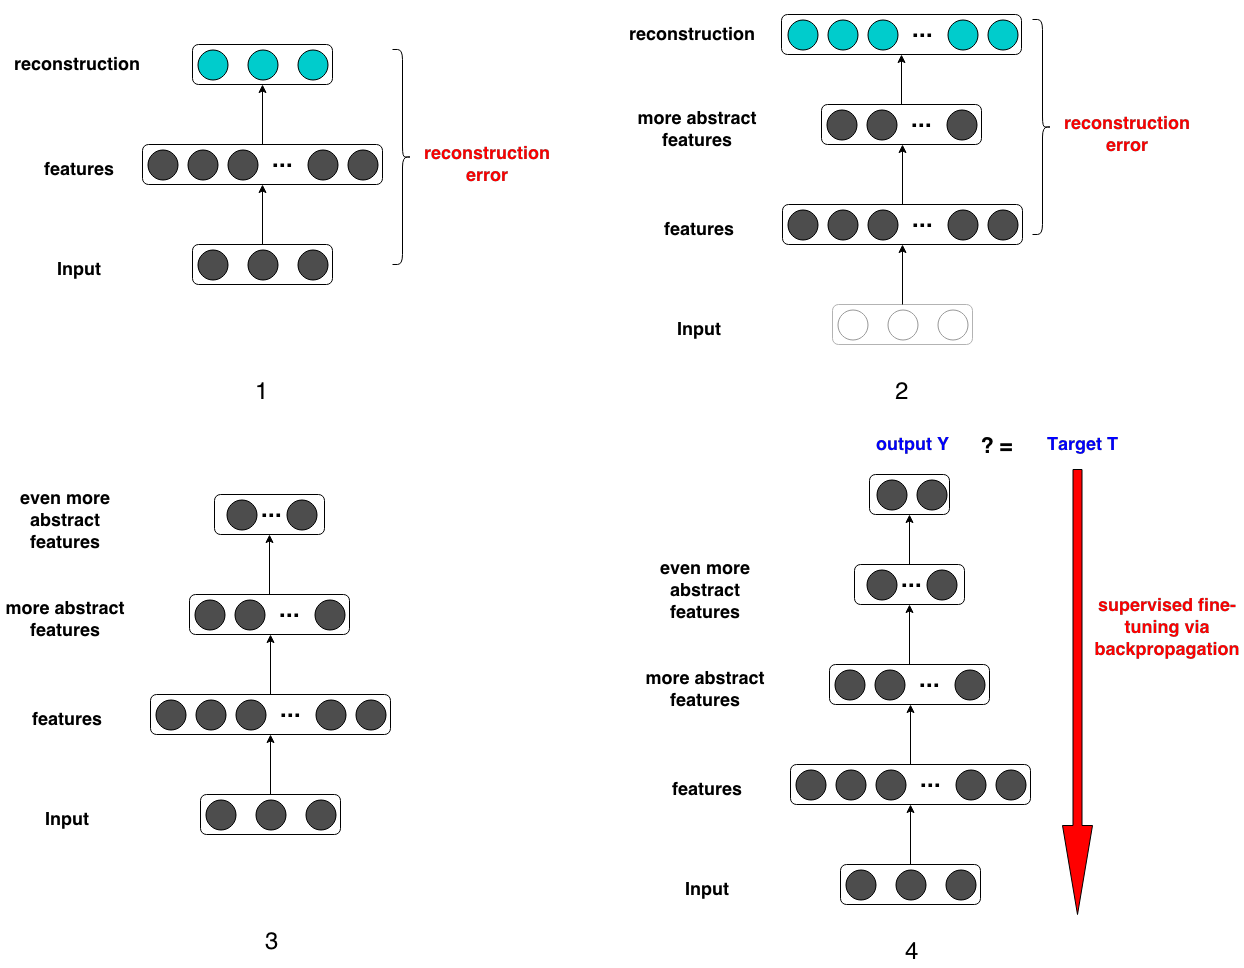
\includegraphics[width=0.9\linewidth]{layerwisewhole.png}
% % 	    \begin{columns}
% % 	     \column{4in}
% % 		\begin{figure}
% % 		 \subfigure{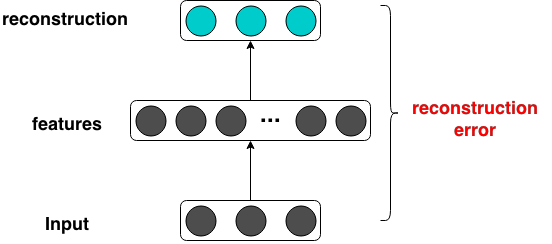
\includegraphics[width=0.4\textwidth]{layerwise1.png}}\\
% % 		 \subfigure{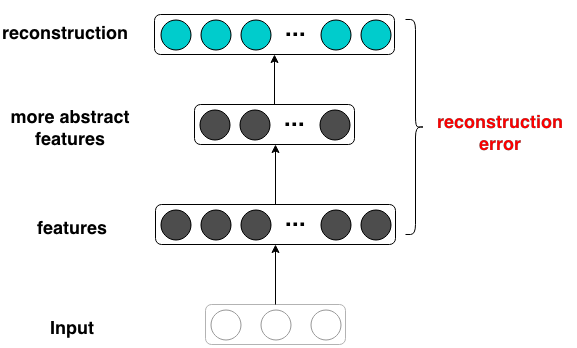
\includegraphics[width=0.4\textwidth]{layerwise2.png}}
% % 		\end{figure}
% % 	     \column{4in}
% % 		 \begin{figure}
% % 		  \subfigure{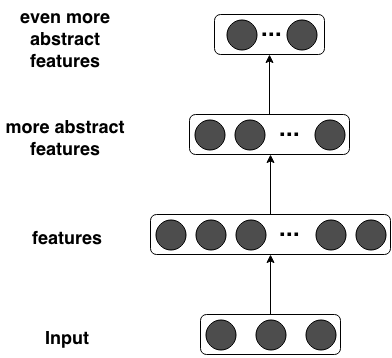
\includegraphics[width=0.4\textwidth]{layerwise3.png}}\\
% % 		  \subfigure{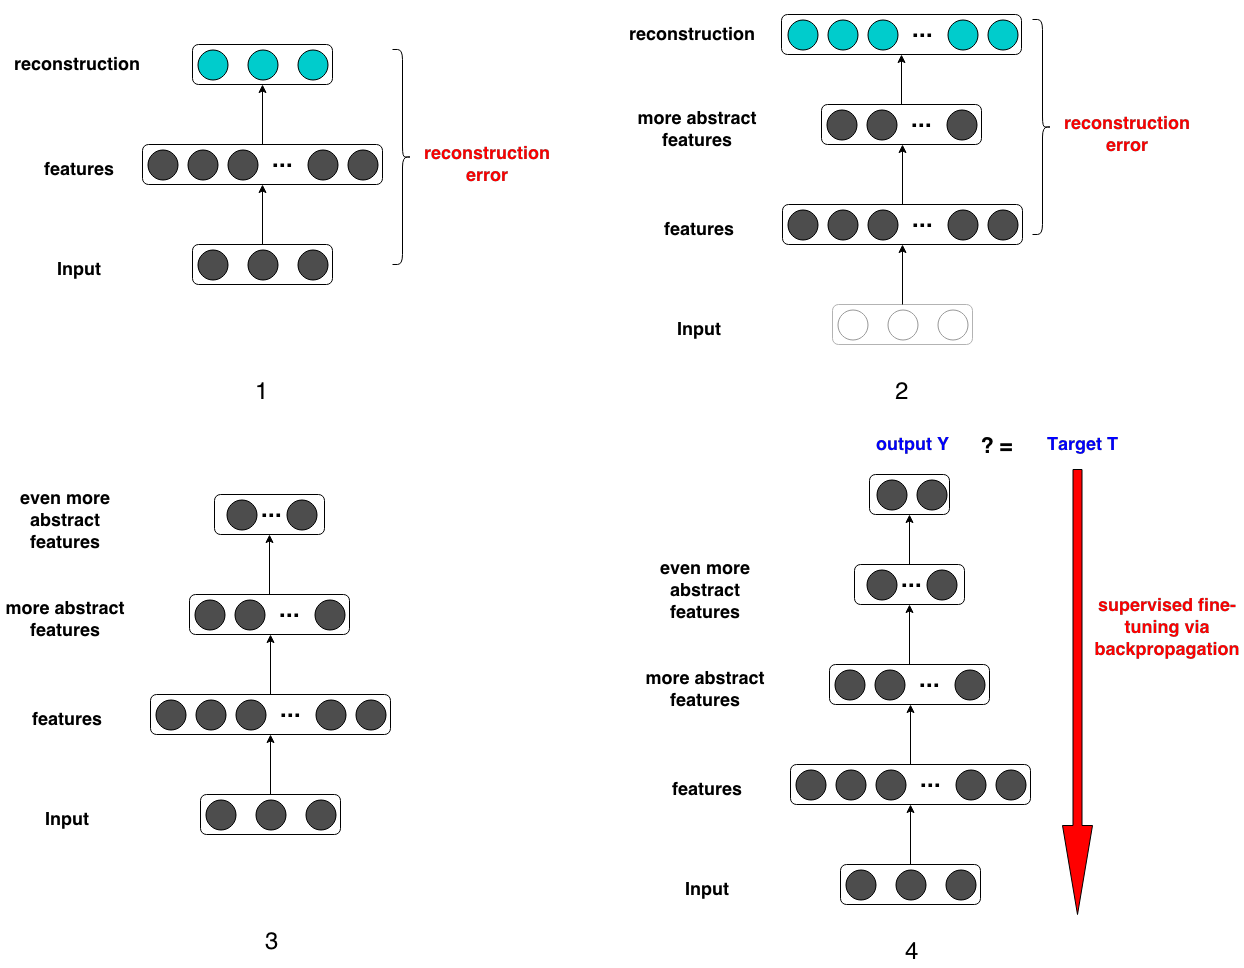
\includegraphics[width=0.4\textwidth]{layerwisewhole.png}}
% % 		 \end{figure}
% % 	      \end{columns}
% 	\end{frame}
% 
% %%%%%%%%%%%%%%%%%%%%%%%%%
% 
% 	
% 	\begin{frame}[t]{Regularization}
% 		\begin{minipage}[h]{\linewidth}
% 		\txtcolb{Overfitting}
% 			\begin{itemize}
% 				\item Huge amount of parameters in deep network
% 				\item Not enough data for training
% 				\item Poor generalization 
% 			\end{itemize}
% 		\end{minipage}\vspace{5mm}
% 		\visible<2->{
% 		\begin{minipage}[h]{\linewidth}
% 		\txtcolb{Regularization}
% 			\begin{itemize}
% 			\item Add weight penalization $\lambda \left\| \mathbf{w} \right\| _{p}$ to loss function 
% 			      \begin{eqnarray}
% 			      \text{arg}~\underset{\btheta}{\mathrm{min}} \frac{1}{M}\sum_m l(\hat{y}(\x^{(m)};\btheta),y^{(m)}) + \lambda \left\| \mathbf{w} \right\| _{p}\nonumber
% 			      \end{eqnarray}
% 			\item 	In convex optimization:
% 	 		\begin{eqnarray}
% 			\text{arg}~\underset{\btheta}{\mathrm{min}} \frac{1}{M}\sum_m l(\hat{y}(\x^{(m)};\btheta),y^{(m)}),  s.t. \left\|\mathbf{w}\right\|_p \leq C\nonumber
% 			\end{eqnarray}
% 			\end{itemize}
% 		\end{minipage}	
% 		}
% 	\end{frame}
% 	
% % 	\begin{frame}[t]{Regularization}
% % 	\txtcolb{P-Norm}
% % 	\begin{eqnarray}
% % 			      \left\| \mathbf{w} \right\| _{p} := \left( \sum_{i=1}^{n} |w_{i}|^{p} \right) ^{1/p} = \sqrt[p]{|w_1|^p +,..., +|w_n|^p}\nonumber
% % 	\end{eqnarray}
% % 	Widely used: L1- and L2-regularization ($p=1$ and $p=2$)
% % 	\begin{figure}[t]
% % % 	\includegraphics<1>[width=0.7\linewidth]{contoursreg.png}
% % 	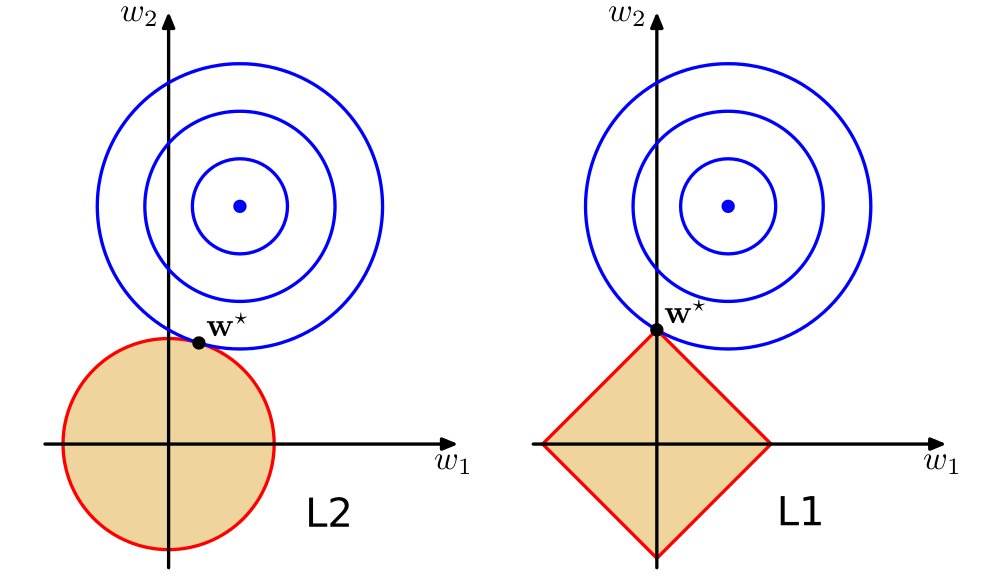
\includegraphics[width=0.7\linewidth]{l1vsl2.png}
% % % 	 \only<1-1>{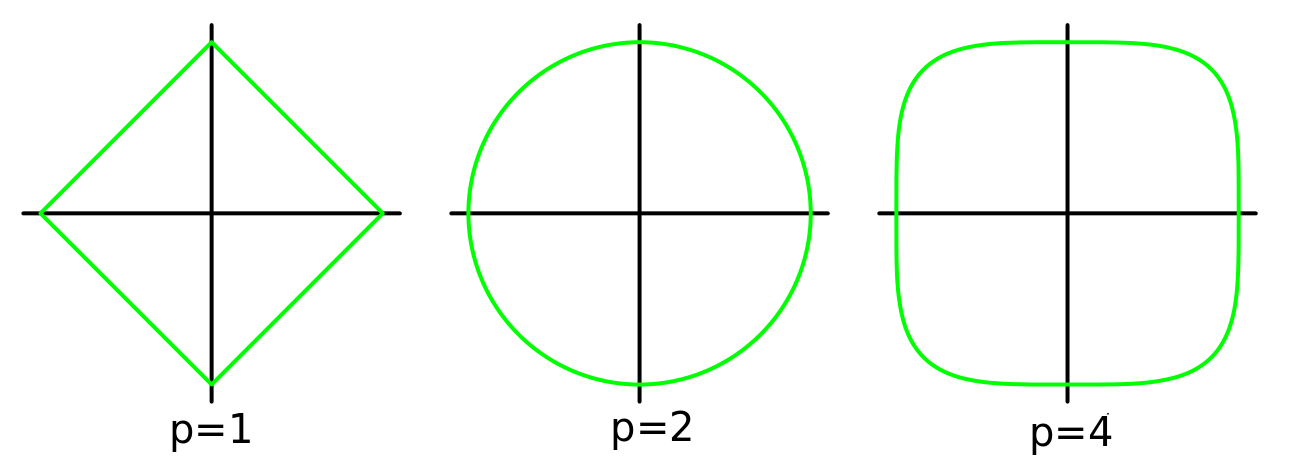
\includegraphics[width=0.7\linewidth]{contoursreg.png}}
% % % 	 \only<2->{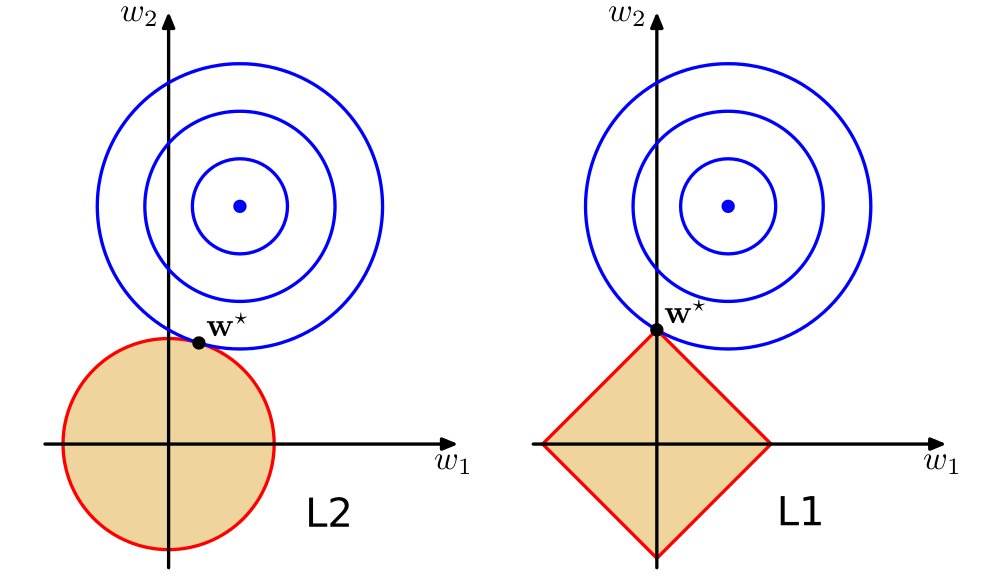
\includegraphics[width=0.7\linewidth]{l1vsl2.png}}
% % 	\end{figure}
% % 
% % 	\end{frame}
% 
% 	
% % %%%%%%%%%%%%%%%%%%%%%%%%%%%%%%%%%%%%%%%%%%%%%%%%%%%%%%%%%%%%%%%%%%%%%%%%%%%%%%%%%%%%%%%%%%%%%%
% 
% 
% % \section{Long Short Term Memory}
% % % 		\begin{frame}[t]{Recurrent Neural Network}
% % % % 			\begin{minipage}[t][][t]{0.48\linewidth}
% % % 			\textcolor{blue}{\Large Concepts of RNN}
% % % 				\begin{itemize}[<+->]
% % % % 				 \itemsep10pt
% % % 				 \item modelling sequential data, emotion in speech .
% % % 				 \item Same Structure as MLP but differs from feed-forward network, enabling
% % % nonlinear mapping
% % % 				 \only<2-2>{
% % % 					\begin{eqnarray}
% % % 						&h_{t} = \mathcal{H}(W_{xh}x_{t}+W_{hh}h_{t-1} + b_{h})\nonumber\\
% % % 						&y_{t} = W_{hy}h_{t} + b_{y}\nonumber
% % % 					\end{eqnarray}
% % % 				 }
% % % 				
% % % 				 \item Feedback connection between previous hidden units and current hidden units, enabling
% % % memory past hidden state.
% % % 				 \item Potentially to model arbitary dynamic system.
% % % 				 \item Trained with \textbf{b}ack\textbf{p}ropagation \textbf{t}hrough \textbf{t}ime (BPTT)
% % % 				 \note{natural extension of BP in FF network}
% % % 				\end{itemize}
% % % % 			\end{minipage}
% % % \vspace{5mm}
% % % % 		\only<1>{\begin{figure}
% % % % 		          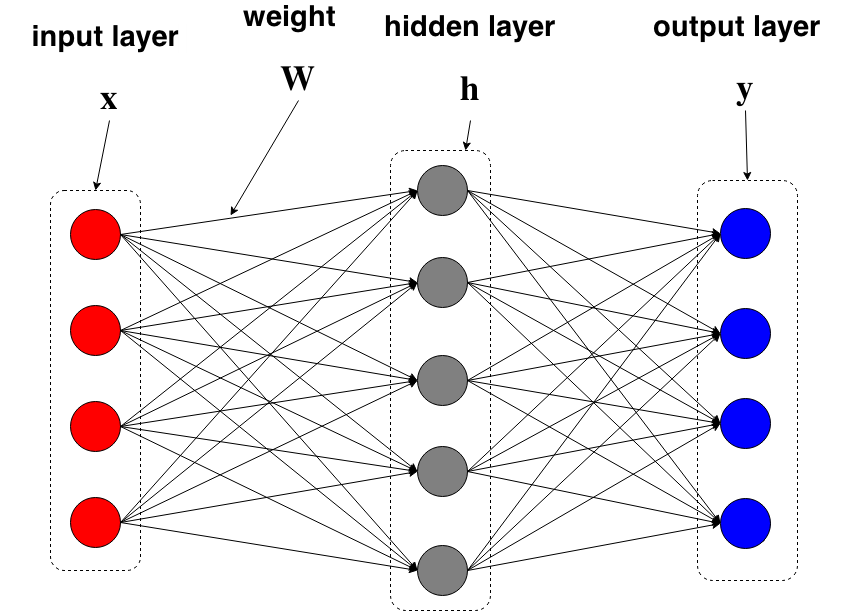
\includegraphics[width=0.5\textwidth]{NeuralNetwork.png}
% % % % 		         \end{figure}
% % % % 
% % % % 		}
% % % 		\end{frame}
% % % 		
% % % 		\begin{frame}[t]{Recurrent Neural Network}
% % % % 			\begin{minipage}[t][][t]{0.48\linewidth}
% % % 			\textcolor{blue}{\Large Concepts of RNN}
% % % 			\begin{minipage}[t]{0.48\linewidth}
% % % 				\only<1>{
% % % 				\begin{figure}[t]
% % % 				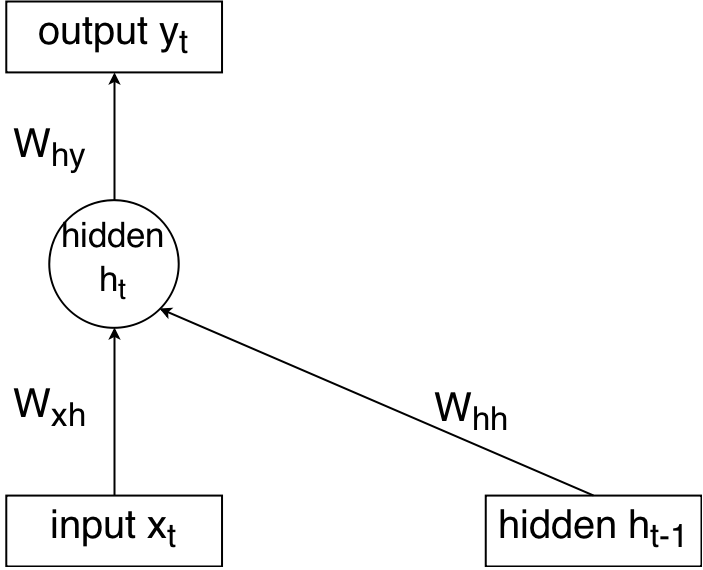
\includegraphics[width=0.8\textwidth]{RNNunit.png}
% % % 				\end{figure}
% % % 				}
% % % 			\end{minipage}\hfill
% % % 			\begin{minipage}[t]{0.48\linewidth}
% % % 				\only<1>{
% % % 				\begin{figure}[t]
% % % 				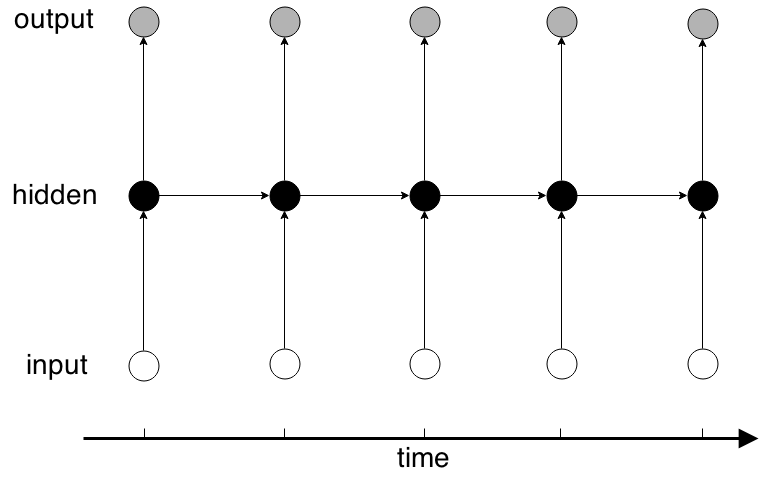
\includegraphics[width=\textwidth]{RNNStruct.png}
% % % 				\end{figure}
% % % 				}
% % % 			\end{minipage}
% % % 
% % % 		\end{frame}
% %     
% %     
% % 
% % 		\begin{frame}[t]{Long Short Term Memory}
% % 		    \only<1-2>
% % 		    {\textcolor{blue}{\Large Problems in RNN}
% % 			\begin{itemize}%[<+->]
% % 			 \item gradient vanishing during backpropagation throught time (BPTT) as time steps increases (>100)
% % 			 \item difficult to capture long-time dependency
% % 			\end{itemize}
% % 		    }
% % 		    \only<2-2>
% % 			{\vspace{5mm} 
% % 			\txtcolb{Long Short Term Memory}\\
% % 			S. Hochreiter and J. Schmidhuber, Lovol. 9, pp. 1735-1780, 1997.\\
% % 			}
% % 		    \only<3->{
% % 		    \includegraphics<3>[scale=0.35]{LSTMstruct.png}
% % % 		    \begin{columns}[T]
% % % 			\column{1.5in}
% % % 			 \includegraphics<4>[width=\linewidth]{LSTMstruct.png}
% % % 			 \only<4->{
% % % 			 \column{1.5in}
% % % 			 \begin{align}
% % % 				  i_{t} &= \sigma (W_{xi}x_{t} + W_{hi}h_{t-1} + W_{ci}c_{t-1} +b_{i})\nonumber\\
% % % 				  f_{t} &= \sigma (W_{xf}x_{t} + W_{hf}h_{t-1} + W_{cf}c_{t-1} +b_{f})\nonumber\\
% % % 				  c_{t} &= f_{t}c_{t-1} + i_{t}\mathrm{tanh}(W_{xc}x_{t} + W_{hc}h_{t-1} + b_{c})\nonumber\\
% % % 				  o_{t} &= \sigma (W_{xo}x_{t} + W_{ho}h_{t-1} + W_{co}c_{t} +b_{o})\nonumber\\
% % % 				  h_{t} &= o_{t}\mathrm{tanh} (c_{t})\nonumber
% % % 			 \end{align}
% % % 			 } 
% % % 		      \end{columns}
% % 		     } 
% % 		\end{frame}
% % 		
% % 		\begin{frame}[t]{Long Short Term Memory}
% % 		\textcolor{blue}{\Large Features in LSTM}
% % 		      \begin{itemize}
% % 			\item gates are trained to learn when it shoud be open/closed. 
% % 			\item Constant Error Carousel
% % 			\item preserve long-time dependency by maintaining gradient over time. 
% % 		      \end{itemize}
% % 		      
% % 		      \begin{figure}
% % 			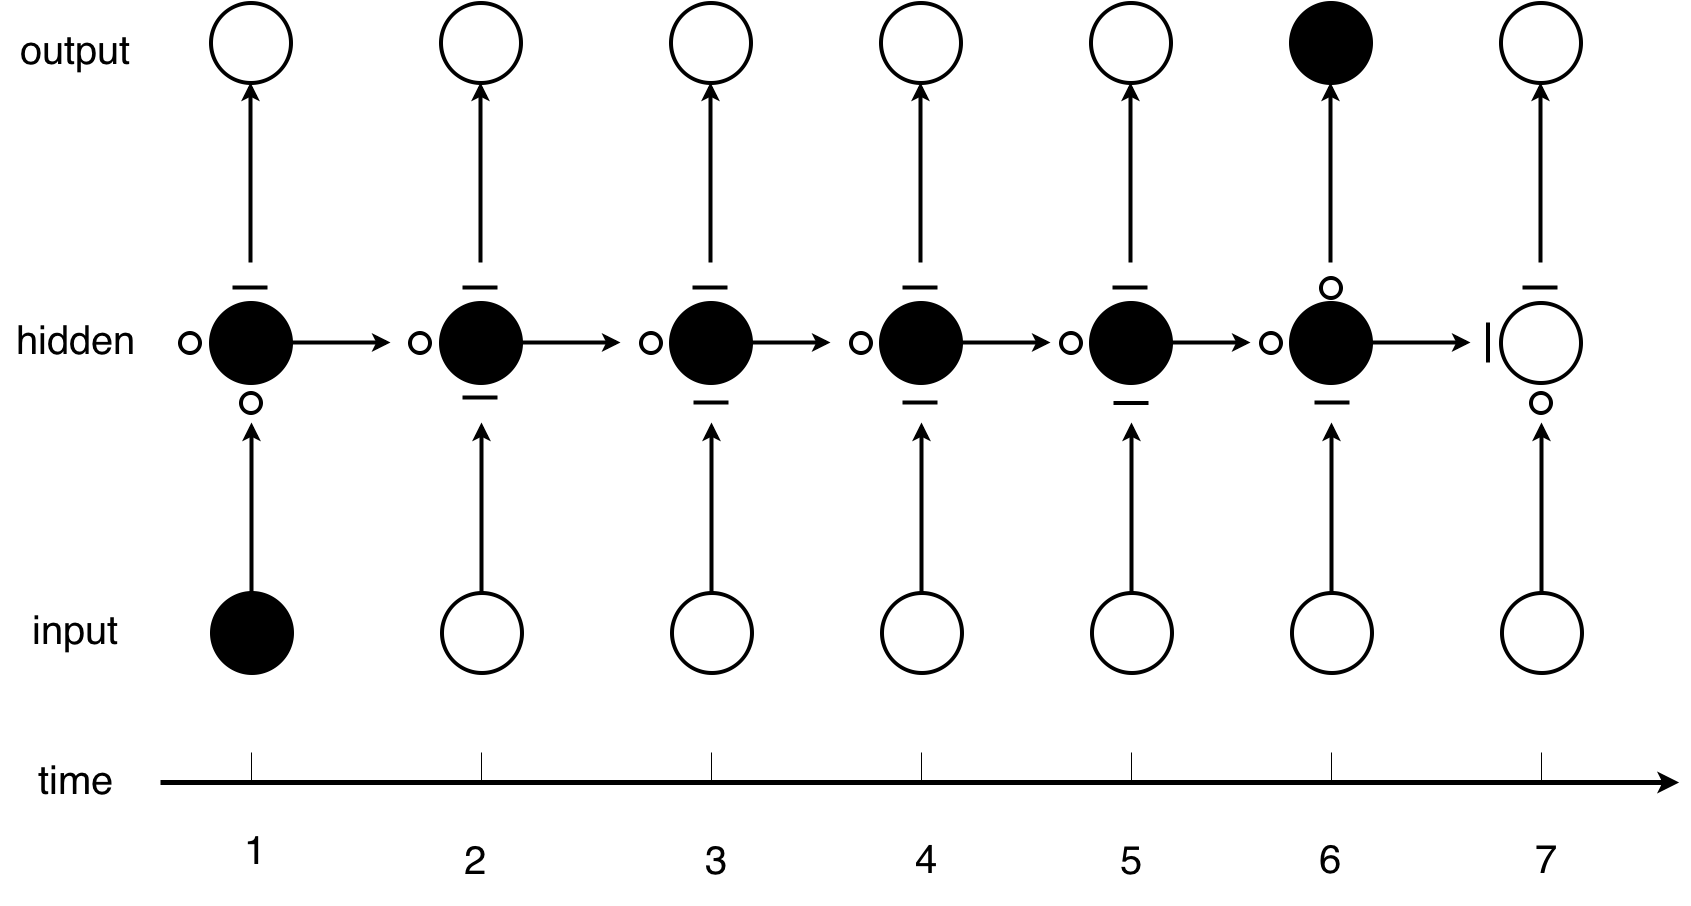
\includegraphics[width=0.75\textwidth]{LSTMGraV.png}
% % 			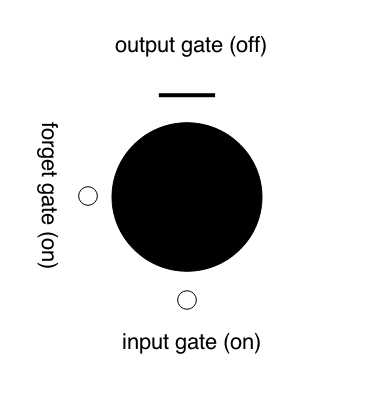
\includegraphics[width = 0.25\textwidth]{GatePos.png}
% % 		      \end{figure}
% % 
% % 
% % 		\end{frame}
% % 		
% % 		
% % % % %%%%%%%%%%%%%%%%%%%%%%%%%%%%%%%%%%%%%%%%%%%%%%%%%%%%%%%%%%%%%%%%%%%%%%%%%%%%%%%%%%%%%%%%%


\section{Experiments}
	\begin{frame}[t]{Experiment Setup}
	  \txtcolb{EmoDB Database}
	  \begin{figure}
		    \begin{tabular}{l|*{4}{c}|c}
			  & Joy & Neutral & Sadness & Anger & Total\\
			\hline
			No. of sentences &71	&79	&62	&127 & 339\\
			\hline
		    Percent (\%) &21 & 23.2 & 18.3& 37.5 & 100
		    \end{tabular}
	  \end{figure}
	  \txtcolb{Data Structure}
	  \begin{figure}
	   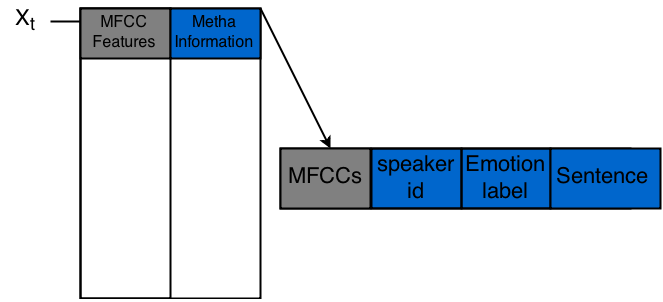
\includegraphics[scale=0.3]{DataStruct.png}
	  \end{figure}
	\end{frame}

	
	\begin{frame}[t]{Experiment Result}
		      \only<2>
	      {
	      \begin{table}[htbp]\centering
	      \centering
	      Confusion matrix of CRBM-DNN result.\\
	      \vspace{10mm}
	      \begin{tabular*}{\linewidth}{@{\extracolsep{\fill}} cl*{4}c @{}}
		  \toprule
		  & \multicolumn{5}{c}{\textit{{Classfied}}} \\[1ex]
	      %     \midrule
		  \multirow{5}{*}{\textit{True}}
		  & & Joy & Neutral & Sadness & Anger \\
	      %     \cmidrule{2-12}
		  & Joy             &\textcolor{red}{57.7\%} &1.4\%   		  & 0.0\%		& 40.8\%\\
		  & Neutral         & 17.7\%			&\textcolor{red}{54.4\%} &25.3\%   	&2.5\%     \\
	      %     \rot{\rlap{~\textit{{True}}}}
		  & Sadness         &1.6\%			&27.9\%   		  &\textcolor{red}{70.5\%}   &0.0\%    \\
		  & Anger           & 39.4\%			&1.6\%  		  &0.0\%   	&\textcolor{red}{59.1\%}    \\
		  \midrule
		  & \multicolumn{5}{c}{recognition rate:59.76\%}\\
		  \bottomrule
	      %     \cmidrule[1pt]{2-12}
		\end{tabular*}
	      \label{tab:CRBMDNN}
	      \end{table}
	      }
	      \only<4>
	      {\begin{table}[htbp]\centering
		\centering
		Confusion matrix of CRBM-LSTM result.\\
		\vspace{10mm}
		      \begin{tabular*}{\linewidth}{@{\extracolsep{\fill}} cl*{4}c @{}}
			  \toprule
			  & \multicolumn{5}{c}{\textit{{Classfied}}} \\[1ex]
		      %     \midrule
			  \multirow{5}{*}{\textit{True}}
			  & & Joy & Neutral & Sadness & Anger \\
		      %     \cmidrule{2-12}
			  & Joy             &\textcolor{red}{11.3\%} &9.9\%   		  &   2.8\%	&    76.1\%\\
			  & Neutral         & 0.0\%			&\textcolor{red}{72.2\%} &17.7\%   	&10.1\%     \\
		      %     \rot{\rlap{~\textit{{True}}}}
			  & Sadness         &0.0\%			&4.8\%   		  &\textcolor{red}{88.7\%}   &6.5\%    \\
			  & Anger           & 0.8\%			&1.6\%  		  &0.0\%   	&\textcolor{red}{97.6\%}    \\
			  \midrule
			  & \multicolumn{5}{c}{recognition rate: 71.98\%}\\
			  \bottomrule
		      %     \cmidrule[1pt]{2-12}
			\end{tabular*}
		\label{tab:CRBMLSTM}
		\end{table}
	      }
	      \only<6>
	      {
	      \begin{table}[htbp]\centering
	      \centering
	      Confusion matrix of LSTM-Rectifier result.\\
	      \vspace{10mm}
		      \begin{tabular*}{\linewidth}{@{\extracolsep{\fill}} cl*{4}c @{}}
			  \toprule
			  & \multicolumn{5}{c}{\textit{{Classfied}}} \\[1ex]
		      %     \midrule
			  \multirow{5}{*}{\textit{True}}
			  & & Joy & Neutral & Sadness & Anger \\
		      %     \cmidrule{2-12}
			  & Joy             &\textcolor{red}{57.7\%} &7.0\%   		  &   0.0\%	&    35.2\%\\
			  & Neutral         &6.3\%			&\textcolor{red}{86.1\%} &6.3\%   	&1.3\%     \\
		      %     \rot{\rlap{~\textit{{True}}}}
			  & Sadness         &0.0\%			&6.6\%   		  &\textcolor{red}{93.4\%}   &0.0\%    \\
			  & Anger           & 8.7\%			&0.0\%  		  &0.0\%   	&\textcolor{red}{91.3\%}    \\
			  \midrule
			  & \multicolumn{5}{c}{recognition rate: 83.43\%}\\
			  \bottomrule
		      %     \cmidrule[1pt]{2-12}
			\end{tabular*}
	      \label{tab:LSTMRec}
	      \end{table}
	      }
		\begin{minipage}[t]{\linewidth}
		\begin{itemize}
		  \item<only@1> CRBM-DNN 
		  \item<only@3> CRBM-LSTM
% 		  \item<only@3> LSTM
		  \item<only@5> LSTM with rectifier units
		\end{itemize}
		\end{minipage}\hspace{5mm}
		
		\begin{minipage}[t]{\linewidth}
		    \begin{figure}[b]
		    \only<1>{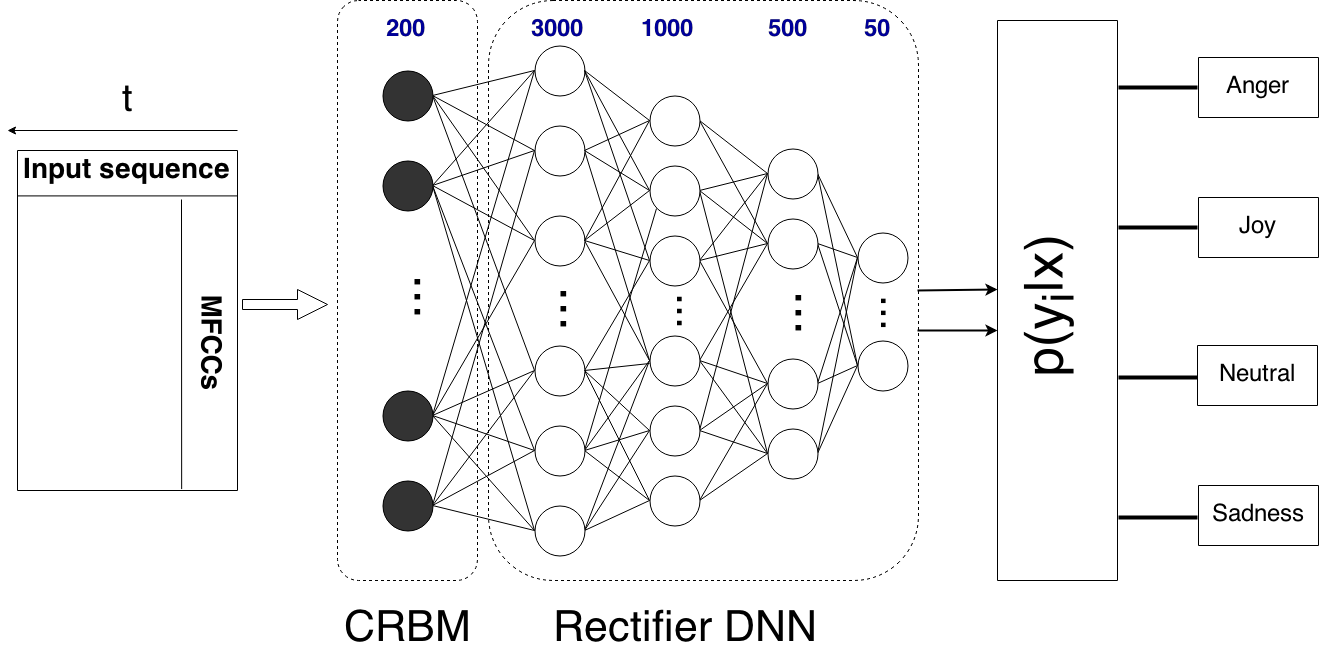
\includegraphics[width=\linewidth]{CRBMDNN.png}}
		    \only<3>{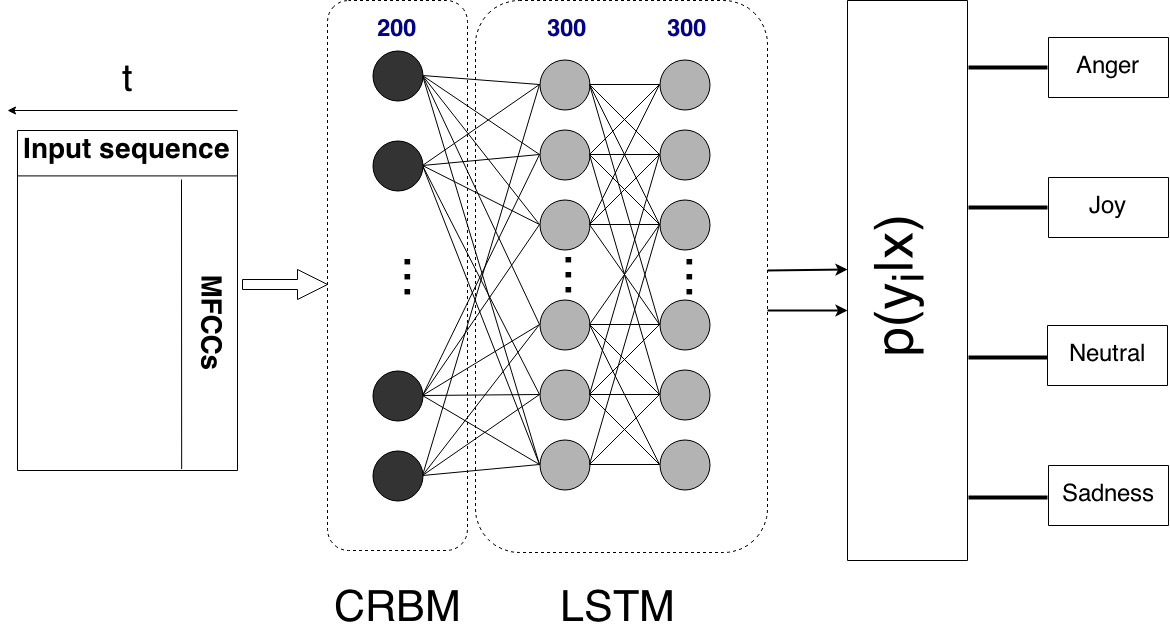
\includegraphics[width=.9\linewidth]{CRBMLSTM.png}}
% 		    \only<3>{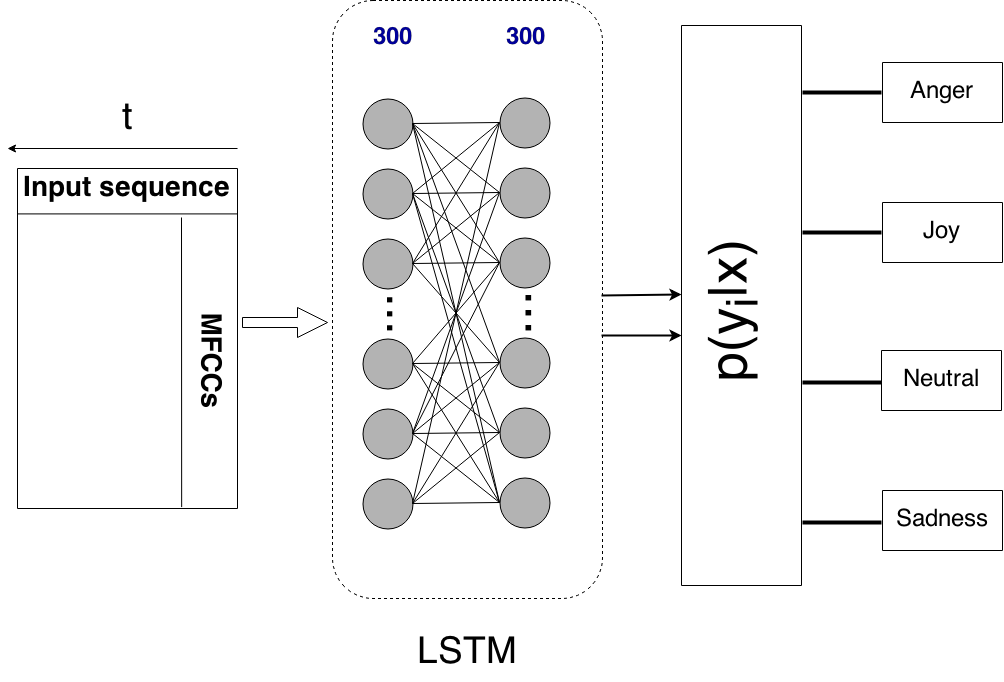
\includegraphics[width=.8\linewidth]{LSTMpure.png}}
		    \only<5>{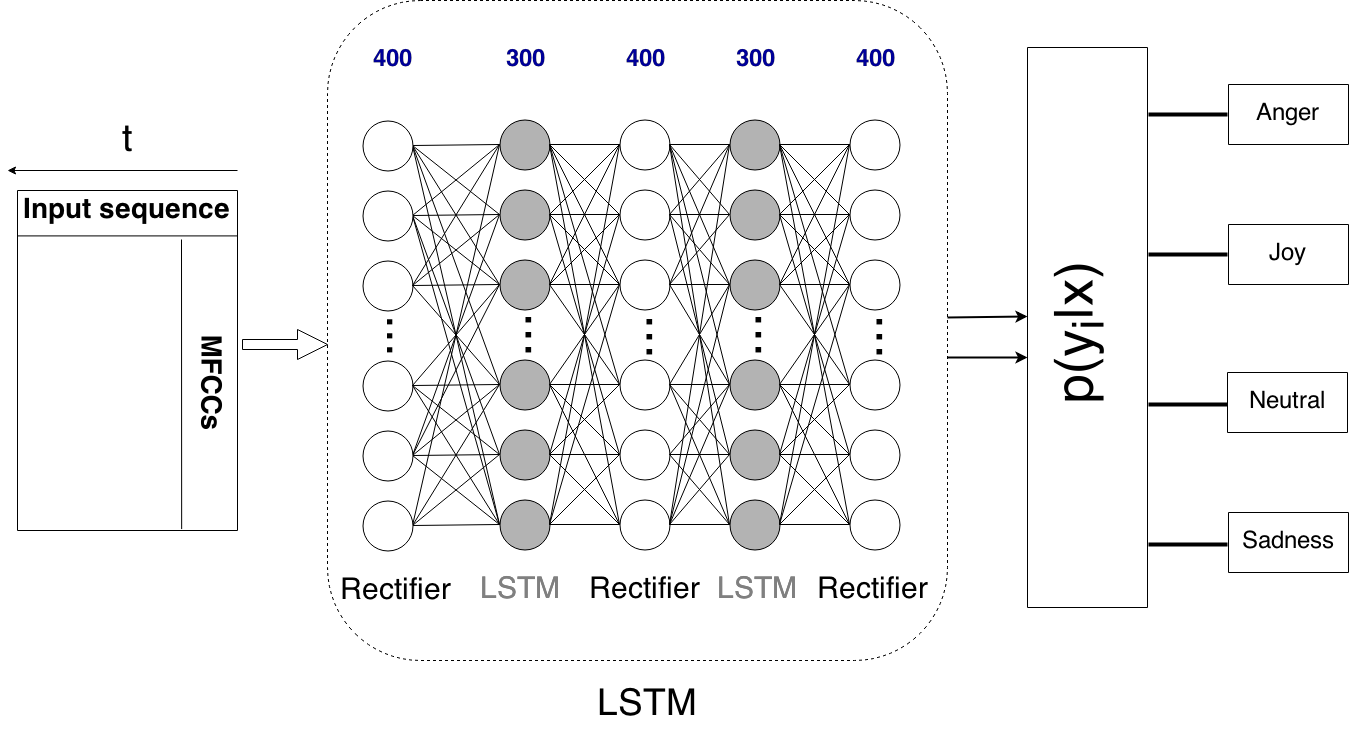
\includegraphics[width=\linewidth]{LSTM.png}}
		  \end{figure}
		  
		\end{minipage}

	\end{frame}
	
% 	\begin{frame}[t]{Result}
% 	      \only<1>
% 	      {
% 	      \begin{table}[htbp]\centering
% 	      \centering
% 	      Confusion matrix of CRBM-DNN result.\\
% 	      \vspace{10mm}
% 	      \begin{tabular*}{\linewidth}{@{\extracolsep{\fill}} cl*{4}c @{}}
% 		  \toprule
% 		  & \multicolumn{5}{c}{\textit{{Classfied}}} \\[1ex]
% 	      %     \midrule
% 		  \multirow{5}{*}{\textit{True}}
% 		  & & Joy & Neutral & Sadness & Anger \\
% 	      %     \cmidrule{2-12}
% 		  & Joy             &\textcolor{red}{57.7\%} &1.4\%   		  & 0.0\%		& 40.8\%\\
% 		  & Neutral         & 17.7\%			&\textcolor{red}{54.4\%} &25.3\%   	&2.5\%     \\
% 	      %     \rot{\rlap{~\textit{{True}}}}
% 		  & Sadness         &1.6\%			&27.9\%   		  &\textcolor{red}{70.5\%}   &0.0\%    \\
% 		  & Anger           & 39.4\%			&1.6\%  		  &0.0\%   	&\textcolor{red}{59.1\%}    \\
% 		  \midrule
% 		  & \multicolumn{5}{c}{recognition rate:59.76\%}\\
% 		  \bottomrule
% 	      %     \cmidrule[1pt]{2-12}
% 		\end{tabular*}
% 	      \label{tab:CRBMDNN}
% 	      \end{table}
% 	      }
% 	      \only<2>
% 	      {\begin{table}[htbp]\centering
% 		\centering
% 		Confusion matrix of CRBM-LSTM result.\\
% 		\vspace{10mm}
% 		      \begin{tabular*}{\linewidth}{@{\extracolsep{\fill}} cl*{4}c @{}}
% 			  \toprule
% 			  & \multicolumn{5}{c}{\textit{{Classfied}}} \\[1ex]
% 		      %     \midrule
% 			  \multirow{5}{*}{\textit{True}}
% 			  & & Joy & Neutral & Sadness & Anger \\
% 		      %     \cmidrule{2-12}
% 			  & Joy             &\textcolor{red}{11.3\%} &9.9\%   		  &   2.8\%	&    76.1\%\\
% 			  & Neutral         & 0.0\%			&\textcolor{red}{72.2\%} &17.7\%   	&10.1\%     \\
% 		      %     \rot{\rlap{~\textit{{True}}}}
% 			  & Sadness         &0.0\%			&4.8\%   		  &\textcolor{red}{88.7\%}   &6.5\%    \\
% 			  & Anger           & 0.8\%			&1.6\%  		  &0.0\%   	&\textcolor{red}{97.6\%}    \\
% 			  \midrule
% 			  & \multicolumn{5}{c}{recognition rate: 71.98\%}\\
% 			  \bottomrule
% 		      %     \cmidrule[1pt]{2-12}
% 			\end{tabular*}
% 		\label{tab:CRBMLSTM}
% 		\end{table}
% 	      }
% % 	      \only<3>
% % 	      {
% % 	      \begin{table}[htbp]\centering
% % 	      \centering
% % 	      Confusion matrix of pure LSTM result.\\
% % 	      \vspace{10mm}
% % 		      \begin{tabular*}{\linewidth}{@{\extracolsep{\fill}} cl*{4}c @{}}
% % 			\toprule
% % 			& \multicolumn{5}{c}{\textit{{Classfied}}} \\[1ex]
% % 		    %     \midrule
% % 			\multirow{5}{*}{\textit{True}}
% % 			& & Joy & Neutral & Sadness & Anger \\
% % 		    %     \cmidrule{2-12}
% % 			& Joy             &\textcolor{red}{66.2\%} &4.2\%   		  &   0.0\%	&    29.6\%\\
% % 			& Neutral         &6.3\%			&\textcolor{red}{79.7\%} &10.2\%   	&3.8\%     \\
% % 		    %     \rot{\rlap{~\textit{{True}}}}
% % 			& Sadness         &0.0\%			&19.7\%   		  &\textcolor{red}{80.3\%}   &0.0\%    \\
% % 			& Anger           & 12.6\%			&0.8\%  		  &0.0\%   	&\textcolor{red}{86.6\%}    \\
% % 			\midrule
% % 			& \multicolumn{5}{c}{recognition rate: 81.59\%}\\
% % 			\bottomrule
% % 		    %     \cmidrule[1pt]{2-12}
% % 		      \end{tabular*}
% % 	      \label{tab:pureLSTM}
% % 	      \end{table}
% % 
% % 	      }
% 	      \only<3>
% 	      {
% 	      \begin{table}[htbp]\centering
% 	      \centering
% 	      Confusion matrix of LSTM-Rectifier result.\\
% 	      \vspace{10mm}
% 		      \begin{tabular*}{\linewidth}{@{\extracolsep{\fill}} cl*{4}c @{}}
% 			  \toprule
% 			  & \multicolumn{5}{c}{\textit{{Classfied}}} \\[1ex]
% 		      %     \midrule
% 			  \multirow{5}{*}{\textit{True}}
% 			  & & Joy & Neutral & Sadness & Anger \\
% 		      %     \cmidrule{2-12}
% 			  & Joy             &\textcolor{red}{57.7\%} &7.0\%   		  &   0.0\%	&    35.2\%\\
% 			  & Neutral         &6.3\%			&\textcolor{red}{86.1\%} &6.3\%   	&1.3\%     \\
% 		      %     \rot{\rlap{~\textit{{True}}}}
% 			  & Sadness         &0.0\%			&6.6\%   		  &\textcolor{red}{93.4\%}   &0.0\%    \\
% 			  & Anger           & 8.7\%			&0.0\%  		  &0.0\%   	&\textcolor{red}{91.3\%}    \\
% 			  \midrule
% 			  & \multicolumn{5}{c}{recognition rate: 83.43\%}\\
% 			  \bottomrule
% 		      %     \cmidrule[1pt]{2-12}
% 			\end{tabular*}
% 	      \label{tab:LSTMRec}
% 	      \end{table}
% 	      }
% 	\end{frame}


% 
\section{Conclusion and Outlook}
      \begin{frame}[t]{Conclusion}
	  \begin{itemize}
	  \itemsep10pt
	  \item<1-> Capturing long-term dependencies is necessary for speech emotion recognition
	  \item<1-> CRBM-DNN is inappropriate for speech emotion recognition (ER: $40.24\%$)
	  \item<1-> CRBM can capture non-temporal and temporal dependencies, but only short term
	  \only<3->{\item Frame-based classification can also reach good result}
		\only<3->
		{\vspace{5mm}
		\begin{itemize}
		 \itemsep10pt
		 \item CRBM-LSTM $71.98\%$
% 		 \item LSTM $81.59\%$
		 \item LSTM with rectifier layers $83.43\%$
		 \item Sentence-based model SVM $84.26\%$ (Tobias Gruber 2014)
		\end{itemize}
		}
	  \end{itemize}
	  
	  \only<2-2>{
		    \begin{tabular*}{\linewidth}{@{\extracolsep{\fill}} cl*{4}c @{}}
		  %     & \multicolumn{5}{c}{\textit{\tiny{Classfied}}} \\[1ex]
		      \toprule
		      &Model & Temporal Dependency & Memory & Generaltive \\
		      \midrule
		  %     \cmidrule{2-12}
		      & DNN		& -	&-	& -	\\
		      & RBM             	& - 	& - 	&  \OK   \\
		      & CRBM         	& \OK 	& 2-5 	& \OK     \\
		      & AE         	& - 	& -  	&  - 	   \\
		      & RNN           	& \OK 	& 1-100	&  -	  \\
		      & LSTM		& \OK	& 1-1000& -	\\
		      \bottomrule
		  %     \cmidrule[1pt]{2-12}
		    \end{tabular*}
		    }
      \end{frame}

%       
      \begin{frame}[t]{Outlook}
	  \begin{itemize}
	   \itemsep15pt
	   \item Stacking CRBM to form deep belief network
% 	   \item Train CRBM with more/larger database 
	   \item Second order optimization to speed up learning process, e.g. Newton methods
	   \item Bi-directional LSTM
	  \end{itemize}

      \end{frame}

      \begin{frame}{End}
	\begin{minipage}[c]{\linewidth}
	\centering
	\textbf{\Huge Thank You!}
	\end{minipage}
      \end{frame}
 \begin{frame}[t,plain]
	\titlepage
\end{frame}


 \end{document}




\end{frame}

\begin{frame}
 The content of this talk can be divided into following parts. Firstly the foundation of emotion recognition is shortly introduced which followed by second chapter to talk about CRBM in detail. And, in the third chapter i going to give a introduction to deep neural network regarding its basic structure and functions and how they are trained. Afterwards the result of this work is showed. Finally i am going to draw a short conclusion and give a outlook of the future research. 
\end{frame}

\begin{frame}
 MFCC is one of the most commonly used features in speech emotion recognition.\\
 THe ...spectrum is calcuated ... and tranformed with the following equation to mel-scale in order to ....\\
\end{frame}


\begin{frame}
 The framework of emotion recognition is illustrated in the figure ...\\
 Then those are the foundation of this work and in the next we are going to talk about CRBM
\end{frame}


\begin{frame}
 To extract the emotion representations from the pre-processed MFCC features we build a temporal model named CRBM \\
 In order to understand how this works we firstly take a look at the basic concept called RBM, which...P of a set of training data x, and probability distribution has some parameters to be learned during the training.\\
 RBM is trained in ... \\
 RBM is 
 
\end{frame}

\begin{frame}

\end{frame}

\begin{frame}
 There are several important definitions for understanding RBM. \\
 The first concept is Energy FUnction called E subscript theta, theta denotes the parameter set W,b and c. The energy function defines the structure of the RBM, in other words the is related to how the visible and hidden layer connected with each other.\\
 Then we have a joint distribution P of x,h... , and Z is called partition funtion in order to normaliz e the righ-hand side term sothat it should be a sufficient probability distribution. \\
 from  the definition of the probability distribution we can see that if a higher probability is desired, the energy function should be small. if you are familiar with thermodynamic, you may have heard about Boltzmann distribution which tells us about the state of the system depending on its energy. With lower energy the system is by definition more stable and this idea is borrowed to build RBM. \\
 Another concept Free Energy is defined and will be used in training RBM, we are going to cover this part later. 
\end{frame}

\begin{frame}
 The inference of RBM is quite straightforward it requires only the mathematical calculation where the marginal distribution is calcualted and using Bayes' theorem we can then get the conditional distribution. Then it allows us to calcualte the probability of one particular taking value one given the corresponding input or hidden vector. 
\end{frame}

\begin{frame}
 The RBM is a static model. However the emotion in speech varies over both short and long time period and consequently we need a temporal model to capture those short and long term variation. Therefore before we come to the training of the energy-based model, i am going to introduce an extention of RBM named CRBM\\
 
 The matrix A and B are weight parameters of history visible units to current vis, and history visible units to current hidden units. \\
 Now the visible units are \\
 same as RBM the energy function defines how the units connected with each other, where tilde b is defined as the original bias of visible layer plus the weight matrix A times history visible units, x subscript smaller than t, and the number of history input is specified by N, as shown in the figure intop. similarly case for the hidden bias tilde c. now the parameter set consists of ....and the free energy is also changed. 
\end{frame}

\begin{frame}
 Now let's see how can the energy-based model be trained with MLE. 
 Firstly i am going to introduce the KL-div, which defines the difference between two probability distributions by calculating the follow equation, here the integral is used when we have a continuous distribution and for the case of crbm where the distribution is discrete, the integral is substitued by the sum over x. 
 As previous discussed, we want to use a model to approximate the true data distribution, here the Q...P is .... and the brackets denotes the ...\\
%  [click]
 the first term on the right hand side is the distribution of the data, it can be treated as a constant value during the optimization so the objective remains only the second term
\end{frame}

\begin{frame}
 With the definition of free energy we can now rewrite the likelihood distribution its partial derivative with respect to the parameter set. \\
 if we average the derivative over the data , the objective function ---(how become expectation over ...???\\
 but the problem is that the calculation of the second term on the righthand side requires all configuration of the model which makes it impossible to be done directly, so we need to do sampling sufficiently to approximate the model distribution.
\end{frame}

\begin{frame}
 the technique used for sampling is Gibbs sampling where it performs a markov chain starting from the visible layer at time 0 and the hidden state at time 0 can be calculated with conditional probability, then the visible at time 1 is again calculated with conditional probability.. so this is a full step of Gibbs sampling. \\
%  [click]
 The gibbs step repeats up to k full steps, where k is a pre-defined variable. 
\end{frame}

\begin{frame}
 With k=0, the probability represente the distribution of input data which is independent of parameter set theta.\\
 if Gibbs-steps is performed with big enough k steps e.g. up to infinite then the markov chain is guarantted to converge to ....:
 [click]
 so the model distribution can be approximated with the sampled distribution and the objective function can be rewritten as:
\end{frame}
\begin{frame}
 But in practise we cannot run the steps waiting until the chain converges and instead of optimizing the divergence between 0 step and infinite step, another concept is introduced by Hinton named Contrastive Divergence\\
where the difference of KL between P0 and Pinfinity and KL bet . . P1 and Pinfinity is minimized by calculating the following equation. It has already been known from many experiment that by ruuning one full gibbs step we can already get good approxmation of model distribution\\
From the literature by Hinton, we know that the third term of righthand side is irrelavant in optimization, so we can omit it during the training and simpify the CD.\\
Then we have the updating rule for the parameter set. 
\end{frame}

\begin{frame}
 So in the next we are going to see the Deep Neural Network. The origin of artificial neural network trace back to the 60 and 70 in last century. To immitate how the human brain works, the scientists have used the aritificial neurons and connections to build up the structure of neural network which is illustrated with the figure on the right. The structure shows a single hidden layer feedforward neural network. The data are fed forward from input layer on the bottom and through a hidden layer then to the output layer on the top. \\
 
 the preactivation a of x of the hidden layer can be calculated by multiplying the input vector with weight matrix W superscript 1, adding the bias vector to the product. \\
 
 mapping the preact a  by a non-linear activation function f we can calcualte the activation of the hidden layer. \\
 
 similarly the activation of the output layer hat y is calcualted based on the hidden layer. The output layer can be prediction or classification or fed as input of further network, depending on different activation function. \\
 
 If the number of hidden units is more than 1, then we'll have a multi-layer neural network or DNN.
\end{frame}
\begin{frame}
 Training the neural network is generally done via supervised learning to minimize the empirical risk, which is show in the first equation. It is the averge of loss over a data sequence of size M and plus some regularization term lambda gama of theta. 
 In the optimization the first-order technique gradient descent is most commonly used, where the gradient of each activation wrt to the parameter theta is calculated and backpropagated through the whole network. \\
 In practise the normal batch-gradient requires too much computation so in general the stocha.. and mini ...are applied.
\end{frame}

\begin{frame}
 it has been a big topic in machine learning for quite a long time that how to train a deeper structure sufficiently and effectively, since the deeper the network is, the more useful features can be extracted and the network should be more powerful in classification tasks. But the training of multi-layer neural network via BP suffers from vanishing gradient problem. \\
 Obviously the training time incre...... and most important is that the ....From literature it is recognized that the gradient vanishing is caused by...., so to cope with this problem a technique named .... is applied. \\
 The deep network is trained .... in every step each layer... where hat x is the reconstruction from auto-encoder\\
 after pre-training step the ...entire network is fine-tuned with ...
\end{frame}

\begin{frame}
 With this figure the pre-training step is illustrated in detail. At step 1 the training data is firstly mapped to the hidden layer to extract some features and then mapped again to output layer for reconstruction the input.  After finishing minimize the reconstruction error for the first hidden layer the training is then fed to the pre-trained first hidden layer and from bottom up mapped to the second hidden layer and build the reconstruction of the firsty hidden layer. Now the optimization objective is the second layer, in this case the first hidden layer is treated as input and the recon. error is minimized wrt the first hidden layer. \\
 This steps repeats by feeding the training data directly to the pre-trained layer and minimize the corresponding reconstruction until all the hidden layer of the network is pretrained. Next is to do the supervised training, now BP won't suffers from the gradient vanishing problem since the paramter is good initialized with pre-training step.
\end{frame}

\begin{frame}
 Same as all other models the dnn should face with the overfitting problem. The dnn often have a large size first hidden layer and deep structure, so obviously due to the huge amount of paramters and lack of enough training data the training result may easily end up overfitting and poor generalization. \\
 
 the overfitting problem can be solved by adding an regularization term to the loss function to penalize the weight with a hyper-parameter lambda. In convex optimization adding a regularization term is equivalent to minimize the loss function with constrain on the p-norm of weight parameter. \\
 
 The p-norm is defined as follows.  In practise, using p=1 and p =2 can already prevent overfitting , and the corresponding regularization terms are named l1 and l2 regularization. The contour of l1 and l2 are showen separately in the figure, where the blue line are the contour of unregularized loss function, the origin of the circle indicates the minimum. the region surrounded by red edges are the constrain of L2 on the left and L1 on the right. the optimum value of weight is labeled as w superscript asterisk. From the figure we can see that the L1 regularization can enalbe sparsity of the parameter because the optimal value generally exist at the corner of the rotated square and consequently one of the parameter is zero. 
\end{frame}


\begin{frame}
 So far we have talked about the CRBM and DNN, those belongs to the feedforward network now we are going to a new type of network which is developed from recurrent neural network--- the LSTM. \\
 The ordinary RNN suffers the same vanishing gradient problem during the BPTT, when the recurrent connection goes back to larger time steps in the past, so although it has great potential to model arbitary non-linear dynamic system, but not much real application has seen since its existence. 
 
 Until 1997  xx and xx proposed a new variant of RNN called LSTM and solve the problem of training RNN by designing a special block of the RNN unit showed in this figure.\\
 
The block constains a memory cell ct, whose activation is controlled by three gate units: input gate i forget gate f and the output gate o. \\

The input gate controls when the newly arrived information from visible units is allowed to overwrite the current activation of memory cell, depending on two states of the input gate either "open" or "closed" . The activation of the memory cell is controlled by the forget gate : with gate being switched on, the information in memory cell remains unchanged with the fixed self-connection of weight 1, i.e. information is stored;  while with gate being switched off, the information is discarded and the cell is reset to the initial state. \\
\end{frame}
\begin{frame}
All the gate are trained to learn when it should be open or closed during the propagation.\\
With the forget get The memory cell can keep the information unchanged and this is called constant error carousel
With such the special memory block, LSTM is capable to preserve the long-time dependencie by maintaining the gradients over time
This is the central feature of LSTM. \\
With the figure below, lets see how this works.
At time step 1, the input arrives at the cell, the input gate is on, then it can overwrite the current activation. and the the forget gate is on, so the information is stored by the memory cell, and the output gate is off so it wont be red by other other units.  this was kept until step 6, the output gate on, the information is read by other units ,and then in time step 7 the forget and output is closed, old information is discarded. 
\end{frame}

\begin{frame}
 So much for the deen network model, now we come to the experiment to see the performance of different models.
 For the classification task we used the EmoDB database, which is an online available database provided by TU Berlin. There are in total 7 emotions, and we use only four of them for test the performance of the model. 
\end{frame}

\begin{frame}
 Schluss wort.
\end{frame}




% -----------------------------------------------------------------------------
%

\end{document}